\documentclass[a4paper,12pt]{report}
\usepackage{graphicx}  % For including images
\usepackage{float}     % For controlling figure placement
\usepackage{fancyhdr} % For custom headers and footers
\usepackage{enumitem}
\usepackage{caption}   % For customizing captions
%\usepackage[italian]{babel}
\usepackage{booktabs}
\usepackage{subcaption}
\usepackage{multirow}
\usepackage{hyperref}
\usepackage{geometry}
\usepackage[rightcaption]{sidecap}
\usepackage{algorithm}
\usepackage{algorithmicx}
\usepackage{algpseudocode}
\usepackage{comment}
\usepackage{multirow}
\newcommand\tab[1][1cm]{\hspace*{#1}}
\usepackage{amsmath}
\usepackage{amssymb}
\usepackage{fontspec}
\usepackage{appendix}
\usepackage{tabularx}
\usepackage{setspace} % Pacchetto per gestire l'interlinea
\usepackage{tikz}
\usepackage{listings}
\usepackage{siunitx}
\usepackage{xcolor}
\usepackage{csquotes} % AGGIUNGI QUESTO per correggere il warning di babel
\usepackage[skins]{tcolorbox}
\definecolor{notaarancio}{HTML}{F77F00}

\newtcolorbox{nota}[1][]{
	empty,
	title={\textbf{Note: #1}},
	attach boxed title to top left,
	boxed title style={empty, size=minimal, bottom=1.5mm},
	coltitle=notaarancio,
	fonttitle=\bfseries\itshape,
	borderline west={2.5pt}{0pt}{notaarancio!35},
	colback=white,
	left=4mm,
	top=0mm,
	bottom=0mm,
	fontupper=\small,
	parbox=false
}

\definecolor{exampleceleste}{RGB}{55, 155, 255}

\newtcolorbox{example}[1][]{
	empty,
	title={\textbf{Example: #1}},
	attach boxed title to top left,
	boxed title style={empty, size=minimal, bottom=1.5mm},
	coltitle=exampleceleste,
	fonttitle=\bfseries\itshape,
	borderline west={2.5pt}{0pt}{exampleceleste!35},
	colback=white,
	left=4mm,
	top=0mm,
	bottom=0mm,
	fontupper=\small,
	parbox=false
}


\renewcommand{\listfigurename}{Figure Listing}
\renewcommand{\lstlistlistingname}{Code Listing}



\usepackage{amsthm}

\newtheorem{theorem}{Theorem}[section]
\newtheorem{lemma}[theorem]{Lemma}


\pagestyle{fancy}
\fancyhf{} % Clear all header and footer fields
\fancyhead[L]{\nouppercase{\leftmark}} % Left section name in header
%\fancyhead[R]{G4} % Left section name in header
\fancyfoot[C]{\thepage} % Centered page number in footer

\usepackage[
backend=biber,
style=numeric,
sorting=nty
]{biblatex}

% CORREZIONE: Usa \addbibresource invece di \bibliography per BibLaTeX
\addbibresource{biblio.bib}


\setmonofont{UbuntuMono-Regular.ttf}[Path=./, Scale=MatchLowercase]


\definecolor{mGreen}{rgb}{0,0.6,0}
\definecolor{mGray}{rgb}{0.5,0.5,0.5}
\definecolor{mPurple}{rgb}{0.58,0,0.82}
\definecolor{backgroundColour}{rgb}{0.95,0.95,0.92}





\lstdefinestyle{mystyle}{
	backgroundcolor=\color{backgroundColour},   
	commentstyle=\color{mGreen},
	keywordstyle=\color{mPurple},
	numberstyle=\tiny\color{mGray},
	stringstyle=\color{mPurple},
	basicstyle=\ttfamily\footnotesize,
	breakatwhitespace=false,         
	breaklines=true,                 
	captionpos=b,                    
	keepspaces=true,                 
	numbers=left,                    
	numbersep=5pt,                  
	showspaces=false,                
	showstringspaces=false,
	showtabs=false,                  
	tabsize=2,
	language=C
}

\lstset{style=mystyle}

\geometry{
	a4paper,
	left=3.5cm, % 3 cm + 0.5 cm for binding
	right=3cm,
	top=3cm,
	bottom=3cm
}


\begin{document}

\begin{titlepage}
    \centering

    {\scshape\huge UNIVERSITY OF SALERNO \par}
    \vspace{1cm}

    {\scshape\large Department of Information and Electrical Engineering, and Applied Mathematics \par}
    \vspace{0.5cm}
    
\vfill
    
    
    
\includegraphics[width=0.5\textwidth]{Misc/logo_standard (1).png}\par
    \vspace{0.5cm} % Add your university's logo here
    
    
    {\scshape\large Master's Degree in Computer Engineering \par}
    \vspace{1.0cm}
    \vfill
    {\huge\bfseries Warehouse Scheduling: Update 8th October\par}
    \vspace{1.0cm}
    
    

    \vfill

    \begin{flushleft}
        \large
        \begin{tabbing}
        	\hspace{8cm} \= \kill
        	\textbf{Supervisor} \> \textbf{Candidate} \\
        	Ch.mo Prof. Francesco Basile \> Gabriele Imparato \\
        	\> \textbf{Serial Nbr.} 0622702508\\
        \end{tabbing}
    \end{flushleft}

    \vfill

    {\large Academic Year 2025/2026\par} % Any additional information like the date
\end{titlepage}

\tableofcontents

\chapter{Introduction}
\subsection{Event-Scheduling Scheme}
Questo approccio si concentra sugli eventi come entità centrali che modificano lo stato del sistema in istanti temporali discreti.

Il simulatore mantiene una lista centrale ordinata chiamata \textbf{Scheduled Event List} (\textbf{SEL}). Ogni elemento della lista è una coppia composta da un tipo di evento e il momento esatto in cui accadrà. Il motore di simulazione funziona estraendo l'evento \textit{più imminente}, portando il tempo globale della simulazione a quel valore ed eseguendo la routine associata a quello specifico evento per aggiornare lo stato del sistema (es. un arrivo o una partenza).

La logica è prettamente legata alle attivazioni temporali e risulta "frammentata". Non esiste una visione globale della vita di un oggetto; ci sono solo blocchi isolati di codice che si attivano quando scatta un determinato clock.

\subsection{Process-Oriented Scheduling Scheme}
Questo approccio sposta il focus dagli eventi alle \textbf{entità} (es. i clienti in una coda, i pezzi in una catena di montaggio o i pacchetti in una rete) che attraversano il sistema.

Un \textit{processo} descrive l'intera sequenza di eventi e intervalli temporali che una singola entità sperimenta durante il suo ciclo di vita all'interno del sistema. Ad esempio:
\begin{enumerate}
	\item Arriva l'entità;
	\item Si controlla che il server è libero;
	\item Si riserva la risorsa;
	\item Attesa per la durata del servizio;
	\item Rilascio della risorsa;
\end{enumerate}

Nella simulazione orientata ai processi, ogni entità si comporta come se fosse un oggetto o un thread indipendente con la propria linea di controllo. Il codice viene scritto dal punto di vista dell'entità, e contiene funzioni che possono "sospendere" temporaneamente l'esecuzione del thread (es. funzioni di time delay o attese condizionate in coda prima di ottenere una risorsa).

\subsubsection{Summary schemes}
Molti linguaggi e software di simulazione moderni (come Arena o SIMSCRIPT citati nel testo) offrono un'interfaccia process-oriented perché è molto più intuitiva per il programmatore. Tuttavia, "sotto il cofano" (a livello di kernel software), spesso traducono tutto in un motore event-scheduling con una SEL centrale, perché è computazionalmente molto più efficiente da eseguire.

\begin{table}[H]
	\centering
	\label{tab:scheduling_schemes}
	\begin{tabularx}{\textwidth}{l X X}
		\toprule
		\textbf{Caratteristica} & \textbf{Event-Scheduling Scheme} & \textbf{Process-Oriented Scheme} \\
		\midrule
		\textbf{Focus principale} & Gli eventi atomici e isolati (Cosa succede al tempo $t$?) & Le entità e il loro ciclo di vita (Cosa fa questo oggetto nel sistema?) \\
		\addlinespace
		\textbf{Punto di vista del codice} & Frammentato in routine basate sul tipo di evento & Sequenziale e lineare per l'entità (simile alla logica di un thread) \\
		\addlinespace
		\textbf{Gestione del tempo} & Salti espliciti basati sulla \emph{Scheduled Event List} (SEL) & Sospensione del processo tramite funzioni di ritardo (\emph{delay}) \\
		\addlinespace
		\textbf{Flessibilità e utilizzo} & Universale, permette di modellare dinamiche molto complesse e arbitrarie & Ideale per sistemi di accodamento e logistica; richiede molte meno righe di codice \\
		\bottomrule
	\end{tabularx}
	
	\caption{Confronto tra Event-Scheduling Scheme e Process-Oriented Scheme.}
\end{table}

\subsection{Colored Petri Net (CPN)}

\subsubsection{Multiset}
Il formalismo matematico alla base dei colore nelle CPN si fonda sui multiset. Un multiset (o multiset non negativo) $\alpha$ definito su un insieme $D$ è una mappatura
\begin{equation}
	\alpha : D \rightarrow \mathbb{Z}
\end{equation}
Oppure riscrivibile come $\alpha : D \rightarrow \mathbb{N}$.

Viene rappresentato formalmente come la sommatoria degli elementi con peso non nullo:
\begin{equation}
	\alpha = \sum_{d\in D} \alpha(d) \oplus d
\end{equation}
In forma vettoriale, corrisponde a un vettore $\alpha =[\alpha(d_1)\alpha(d_2)\cdots \alpha(d_k)]^T \in \mathbb{Z}^k $.\newline

\noindent Operazioni sui multiset:
\begin{itemize}
	\item Somma ($\gamma = \alpha + \beta$): $\forall d \in D: \gamma (d) = \alpha (d) + \beta(d)$;
	\item Differenza ($\gamma = \alpha - \beta$): $\forall d \in D: \gamma (d) = \alpha (d) - \beta(d)$, può risultare negativa anche partendo da multiset non negativi;
	\item Prodotto per scalare ($\gamma = a\alpha$ con $a\in \mathbb{Z}$): $\forall d \in D: \gamma (d) = a\alpha (d)$;
	\item Confronto ($\alpha \le \beta$): $\forall d \in D: \alpha (d) \le \beta(d)$.
\end{itemize}

\subsubsection{Definizione generale di CPN}
Un rete di petri colorata è definita formalmente come una sestupla:
\begin{equation}
	N = (P, T, \text{Pre}, \text{Post}, Cl, Co)
\end{equation}
Dove:
\begin{itemize}
	\item $P$ è l'insieme degli $m$ posti;
	\item $T$ è l'insieme delle $n$ transizioni;
	\item $Cl$ è l'insieme globale dei colori ammissibili;
	\item $Co: P \cup T \rightarrow Cl$ è la \textbf{funzione colore} che associa a ciascun elemento un insieme ordinato e non vuoto di colori ricavati da $Cl$;
	\begin{itemize}
		\item Per un posto $p_i$, $Co(p_i)$ indica i colori possibili per i gettoni (token) contenuti in esso e $u_i$ rappresenta il loro numero;
		\item Per una transizione $t_j$, $Co(t_j)$ indica i possibili colori di occorrenza (o scatto) della transizione e $v_j$ rappresenta il loro numero;
	\end{itemize}
	\item $\text{Pre}$ e $\text{Post}$ sono le matrici di incidenza composte da mappature tra i colori dei posti e i multiset dei colori delle transizioni:
	\begin{equation}
		\text{Pre}(p,t) : Co(p)\rightarrow \mathcal{M}(Co(t))
	\end{equation}
	\begin{equation}
		\text{Post}(p,t) : Co(t)\rightarrow \mathcal{M}(Co(p))
	\end{equation}
	La matrice d'incidenza globale è definita come:
	\begin{equation}
		C = \text{Post} - \text{Pre}
	\end{equation}
\end{itemize}

\subsubsection{Marcatura e stato nelle CPN}
La marcatura $m_i$ di un posto $p_i$ è un multiset non negativo definito su $Co(p_i)$. La funzione associa a ogni potenziale colore di gettone un intero non negativo che indica quanti gettoni di quel colore sono presenti nel posto.

In formato vettoriale colonna di dimensione $u_i$, la componente $h$-esima $m_i(h)$ indica il numero di gettoni di colore $a_{i,h}$ nel posto $p_i$.

La marcatura complessiva delle CPN è un vettore colonna a $m$ dimensioni di multiset:
\begin{equation}
	m = [m_1 \cdots m_m]^T
\end{equation}

\noindent \textbf{Formalismo A: Guardie ed Espressioni sui nodi}
Questo approccio rende i modelli più leggibili dal punto di vista grafico.

\begin{itemize}
	\item \textbf{Funzione colore e transizioni}: la funzione $Co: P \rightarrow Cl$ mappa solo i posti. I colori delle transizioni non sono definiti esplicitamente ma implicitamente tramite funzioni di controllo logico dette \textbf{guardie} ($G(t)$), a valore booleano;
	\item \textbf{Binding}: un assegnamento di valori alle variabili delle espressioni tale per cui $G(t) = 1$ (quindi quando è vera) è chiamato \textit{binding}. L'insieme di tutti i binding possibili per $t$ è denotato come $B(t)$;
	\item Le matrici $\text{Pre}$ e $\text{Post}$ contengono espressioni le cui variabili sono i colori del posto connesso. Quando si applica un binding $\beta$, i valori della marcatura rimossa o aggiunta sono indicati come
	\begin{equation}
		\text{Pre}(\cdot, t)[\beta],
		\text{Post}(\cdot, t)[\beta]
	\end{equation}
	\item \textbf{Abilitazione e scatto}: una transizione $t$ è abilitata per un binding $\beta$ se e solo se la marcatura attuale soddisfa $m \ge \text{Pre}(\cdot, t)[\beta]$. Lo scatto produce una nuova marcatura
	\begin{equation}
		m' = m + \text{Post}(\cdot, t)[\beta] - \text{Pre}(\cdot, t)[\beta] = m + C(\cdot, t)[\beta]
	\end{equation}
\end{itemize}

\noindent \textbf{Formalismo B: Rappresentazione matriciale}
Questo approccio predilige l'algebra lineare ed è particolarmente utile per scopi di ricerca nel controllo di supervisione.
\begin{itemize}
	\item Le entrate delle matrici $\text{Pre}$ e $\text{Post}$ sono interamente costituite da matrici di numeri interi;
	\item $\text{Pre}(p_i, t_j)$ e $\text{Post}(p_i, t_j)$ diventano matrici di dimensioni $u_i \times v_j$ di interi non negativi. Ad esempio, l'elemento generico $\text{Pre}(p_i, t_j)(h, k)$ indica il peso dell'arco dal posto $p_i$ (rispetto al colore del gettone $a_{i,h})$) alla transizione $t_j$ (rispetto al colore di occorrenza $b_{j,k}$);
	\item \textbf{Abilitazione e scatto}: una transizione $t_j$ è abilitata rispetto al colore di occorrenza $b_{j,k}$ alla marcatura $m$ se e solo se $m_i(h) \ge \text{Pre}(p_i, t_j)(h,k)$ per ogni posto $p_i$ e per tutti gli $h= 1,\cdots, u_i$. Lo scatto aggiorna la marcatura per ogni posto secondo l'equazione lineare
	\begin{equation}
		m'_i(h) = m_i(h) + \text{Pre}(p_i, t_j)(h,k) - \text{Post}(p_i, t_j)(h,k) 
	\end{equation}
\end{itemize}

\subsubsection{Controllo di Supervisione e Gestione dei Conflitti}
\begin{itemize}
	\item \textbf{Transizioni controllabili e non controllabili}: l'insieme delle transizioni (o dei singoli colori di occorrenza) è diviso in due sottoinsiemi disgiunti.
	\begin{itemize}
		\item $T_c$, transizioni controllabili che il supervisore può abilitare o disabilitare tramite una variabile booleana $CV$;
		\item $T_{uc}$ transizioni non controllabili, governate esclusivamente dall'impianto;
	\end{itemize}
	Nel formalismo matriciale, un supervisore non può inibire una transizione non controllabile rispetto a un determinato colore;
	\item \textbf{Specifiche di stato (GMEC)}: i vincoli di sicurezza sono spesso espressi tramite Vincoli di Esclusione Mutua Generalizzata (GMEC) che impongono restrizioni sulle marcature legali ammissibili del sistema (es. limitare la capacità dei buffer dei robot o delle macchine nei sistemi flessibili di produzione);
	\item \textbf{Risoluzione dei conflitto}: due transizioni sono in conflitto effettivo se sono entrambe abilitate alla marcatura attuale, ma la quantità di gettoni disponibili non permette lo scatto simultaneo di entrambe. Per rendere deterministico l'avanzamento temporale e logico, la teoria prevede politiche di schedulazione basate su:
	\begin{itemize}
		\item Ordine di priorità statico/predefinito;
		\item Frequenze/probabilità di scatto identiche o stocastiche (routing rates);
		\item Algoritmi o logiche esterne guidate da supervisori basati sullo stato;
	\end{itemize}
	\item \textbf{Gestione del tempo (CTPN)}: le CPN temporizzate introducono una funzione tempo $f$ che associa a ogni binding o colore di occorrenza un ritardo deterministico o stocastico tra l'abilitazione e l'effettivo scatto atomico, permettendo valutazioni di performance (come il calcolo del throughput) attraverso semantiche a servente infinito (infinite server semantic).
\end{itemize}


\chapter{Theoretical foundations and Modeling approaches}
\section{Scheduled Event List}
\label{sec:theory-sel}

Once the warehouse operations have been represented as discrete events, it is
necessary to determine how these events evolve during the simulation. A useful
technique for this purpose is the \textit{Scheduled Event List} (SEL), which
provides a mechanism for managing the events that may occur as the state of the
system changes, following the discrete-event simulation framework described
in~\cite{cassandras2021des}.

The basic idea is to associate each feasible event with the instant of time at
which it is expected to occur. Considering a set of events $E$ and a state space
$X$, at a given state $x \in X$ only a subset of events is feasible. This subset
can be denoted by $\Gamma(x)$. Each feasible event $i \in \Gamma(x)$ is associated
with a clock value $y_i$, representing the amount of time remaining before that
event occurs.

The next event to be executed is therefore the feasible event characterized by
the smallest clock value:

\begin{equation}
	e' = \arg\min_{i \in \Gamma(x)} y_i
\end{equation}


\noindent Consequently, the amount of time spent in the current state is

\begin{equation}
	y^* = \min_{i \in \Gamma(x)} y_i
\end{equation}

\noindent and the simulation time can be updated according to

\begin{equation}
	t' = t + y^*
\end{equation}

\noindent Instead of explicitly maintaining the remaining clock value of every event, the
simulation can store the events together with their scheduled execution times.
The resulting Scheduled Event List can be represented as

\[
L = \{(e_k,t_k)\},
\]

\noindent where $e_k$ represents an event and $t_k$ the corresponding scheduled execution
time.

The evolution of the simulation can then be described as an iterative procedure.
First, the event having the smallest scheduled time is extracted from the SEL
and executed. The simulation clock is advanced to the corresponding event time
and the state of the system is updated. As a consequence of this state change,
some previously scheduled events may no longer be feasible and are therefore
removed from the list, while newly enabled events are inserted. Finally, the SEL
is reordered according to the scheduled execution times before starting the next
iteration.

\begin{figure}[H]
	\centering
	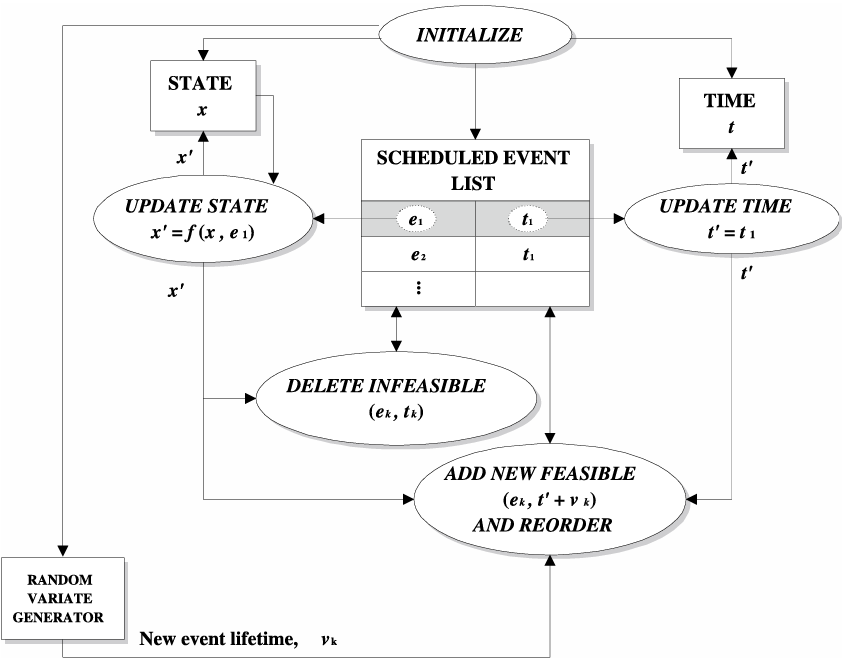
\includegraphics[width=1\linewidth]{imgs/Cap2_teoria/SEL_generalized}
	\caption{Generalized Scheduling Event scheme in computer simulations}
	\label{fig:selgeneralized}
\end{figure}


In the warehouse scheduling problem, this mechanism is particularly useful
because the feasibility of a mission depends on the current state and on the
availability of the resources required to execute it. For example, a loading
operation requiring both a forklift and an operator cannot start until both
resources are available. When another mission is completed and those resources
are released, the state of the system changes and the loading operation may
become feasible and consequently enter the SEL.

The SEL should therefore not be interpreted as a static schedule generated once
at the beginning of the simulation. It is a dynamic structure that evolves
together with the system. This is particularly important when several missions
compete for shared resources, since every completed operation may modify the set
of missions that can subsequently be executed.

In this framework, the SEL provides the temporal mechanism required to determine
\textit{when} events occur. However, an additional model is required to represent
the state of the system, the availability of resources, the dependencies between
operations, and the conditions under which an event becomes feasible. In the
proposed design, admission to a resource queue is an additional scheduling
condition: an enabled operation must also have been admitted before it can
start. Queue replenishment determines which missions enter execution, whereas
the event mechanism orders their simulated state changes. Petri nets
provide a suitable formalism for this purpose.


\section{Petri Nets}

Warehouse operations are characterized by a high degree of concurrency. Several
missions may be active at the same time, different resources may operate
simultaneously, and multiple activities may compete for the same limited
resources. A model used to represent such a system must therefore describe not
only the individual evolution of each mission, but also synchronization,
concurrency, resource availability, and conflicts among different activities.

\textit{Petri nets} (PNs) are a discrete-event modeling formalism particularly
suited to representing these characteristics. A Petri net is a directed bipartite
graph composed of two different types of nodes: \textit{places} and
\textit{transitions}. Places can represent conditions, states, or the availability
of resources, whereas transitions represent events or operations that modify the
state of the system. Places and transitions are connected through directed arcs.
The terminology and firing rules used here follow the formulation
in~\cite{murata1989petri,cassandras2021des}; the use of Petri-net models
for simulation and control is also discussed
in~\cite{basile2007pnetlab}.

The current state of a Petri net is described by its \textit{marking}, namely the
distribution of \textit{tokens} among the places of the net. A transition is
enabled only when its input places contain the tokens required for its execution.
When an enabled transition fires, the corresponding input tokens are consumed
and new tokens are produced in its output places, according to the structure of
the net.

This mechanism naturally represents resource allocation. For example, consider
a warehouse mission that requires both a forklift and an operator. Two places
may represent the availability of these resources. The transition corresponding
to the beginning of the mission can fire only when both places contain the
required tokens. Once the transition fires, the tokens are removed, representing
the fact that the forklift and the operator are currently busy. At the completion
of the mission, another transition can return the tokens to the corresponding
resource-availability places, making them available for subsequent missions.

This representation becomes particularly useful when several missions compete
for the same resources. If two missions require the same forklift, for example,
the availability of a single token prevents both corresponding transitions from
acquiring that resource simultaneously (fig. \ref{fig:pn}). Resource conflicts can therefore be
represented directly through the structure and marking of the net.

\begin{figure}[H]
	\centering
	
	\begin{subfigure}[b]{0.48\textwidth}
		\centering
		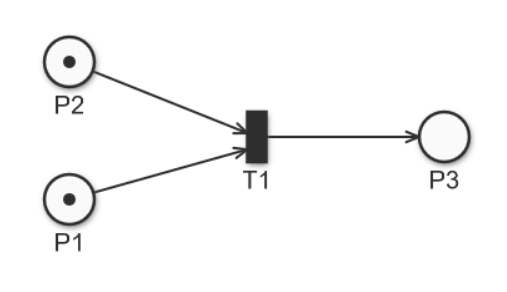
\includegraphics[width=\textwidth]{imgs/Cap2_teoria/pn1.png}
		\caption{Before triggering $t1$}
		\label{fig:pn1}
	\end{subfigure}
	\hfill
	\begin{subfigure}[b]{0.48\textwidth}
		\centering
		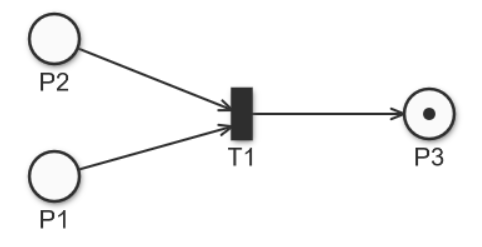
\includegraphics[width=\textwidth]{imgs/Cap2_teoria/pn2.png}
		\caption{After triggering $t1$}
		\label{fig:pn2}
	\end{subfigure}
	
	\caption{Example of petri net transition firing}
	\label{fig:pn}
\end{figure}

\noindent Compared with a representation based exclusively on finite-state machines,
Petri nets provide a natural way to describe several concurrent activities within
the same model. This characteristic is especially relevant in warehouse systems,
where many missions may evolve simultaneously and their execution may depend on
shared resources.

Petri nets can also be represented mathematically through incidence
matrices~\cite{murata1989petri}.
In particular, the \textit{Pre} and \textit{Post} matrices describe the
connections from places to transitions and from transitions to places,
respectively. This representation is particularly useful when the model has to be
automatically generated, simulated, or integrated into an optimization algorithm.

From a mathematical point of view, a Place/Transition Petri Net can be defined
as the four-tuple $N = (P,T,Pre,Post)$ where $P$ is the set of places, $T$ is the set of transitions, while $Pre$ and $Post$ describe the connections between places and transitions.

The structure of the net can also be represented through the incidence matrix

\begin{equation}
	C = Post - Pre
\end{equation}

\noindent The state of the system is represented by the \textit{marking} $m$, which
specifies the number of tokens contained in each place. A transition $t$ is
enabled only if all its input places contain the required number of tokens:

\begin{equation}
	m(p) \geq Pre(p,t),
	\qquad \forall p \in {}^\bullet t
\end{equation}

\noindent When an enabled transition fires, the marking of the Petri Net changes according
to the tokens consumed and produced by the transition. More generally, the
evolution of the marking after a sequence of transition firings can be expressed
through the state equation

\begin{equation}
	m = m_0 + C\sigma
\end{equation}

\noindent where $m_0$ is the initial marking and $\sigma$ is the firing-count vector,
whose elements indicate how many times each transition has fired.

\subsection{Colored Petri Nets}

When the system contains a large number of missions and several similar resources,
a standard Petri-net representation may become increasingly complex. A useful
extension is represented by \textit{Colored Petri Nets} (CPNs), which introduce
different types of tokens, generally referred to as \textit{colors}. The basic
concepts and modeling principles of CPNs are presented
in~\cite{jensen1997coloured}, while their use for discrete-event simulation
and control is discussed in~\cite{basile2007pnetlab}.

The use of colors makes it possible to distinguish different resources or
operational conditions while preserving the general structure of the Petri net.
In a warehouse scenario, for example, different colors can be associated with
different operators and forklifts combination involved in mission execution.
In this way, multiple resources can evolve simultaneously through the same model
without losing information about which specific resource is performing a given
task.

Formally, a Colored Petri Net can be defined as the six-tuple

\[
N=(P,T,Pre,Post,Cl,Co),
\]

\noindent where $P$ is the set of places, $T$ is the set of transitions, $Cl$ is the set
of colors, and $Co : P \cup T \rightarrow 2^{Cl}$ is the color function that associates each place and transition with an ordered
set of admissible colors.

For a place $p_i \in P$, the set of possible token colors can be expressed as

\begin{equation}
	Co(p_i)=\{a_{i,1},a_{i,2},\dots,a_{i,u_i}\}\subseteq Cl,
\end{equation}

\noindent while, for a transition $t_j \in T$, the corresponding set of occurrence
colors is

\begin{equation}
	Co(t_j)=\{b_{j,1},b_{j,2},\dots,b_{j,v_j}\}\subseteq Cl.
\end{equation}

\noindent Unlike a standard Petri Net, in which the marking of a place is represented only
by the total number of tokens, in a CPN the marking must also preserve information
about their colors. Therefore, the marking of a place $p_i$ can be represented
by the vector

\[
m_i =
\begin{bmatrix}
	m_i(1)\\
	m_i(2)\\
	\vdots\\
	m_i(u_i)
\end{bmatrix},
\]

\noindent where $m_i(h)$ represents the number of tokens of color $a_{i,h}$ contained in
place $p_i$. The complete marking of the CPN is consequently obtained by
collecting the markings of all places:

\[
m =
\begin{bmatrix}
	m_1\\
	m_2\\
	\vdots\\
	m_{|P|}
\end{bmatrix}.
\]

\noindent This additional information is particularly useful for warehouse optimization.
For example, if several operators are available, each operator can be associated
with a different token color. When a transition corresponding to a mission fires,
the color involved in that transition identifies the particular resource assigned
to the mission.

As in standard Petri Nets, the structural evolution of the system is described
through the incidence matrix

\[
C = Post - Pre.
\]

\noindent However, in a CPN the entries of the $Pre$ and $Post$ matrices also depend on the colors associated with places and transitions.

Considering a transition $t_j$ with occurrence color $b_{j,k}$, the transition
is enabled only if the required number of tokens of each color is available in
its input places:

\begin{equation}
	m_i(h) \geq Pre(p_i,t_j)(h,k).
\end{equation}

\noindent If the transition fires, the marking is updated according to

\begin{equation}
	m_i'(h)
	=
	m_i(h)
	+
	Post(p_i,t_j)(h,k)
	-
	Pre(p_i,t_j)(h,k).
\end{equation}

\noindent These equations show why the introduction of colors is particularly useful in a
resource-allocation problem. The enabling of a transition does not depend only
on the total availability of resources, but also on the availability of the
specific type or identity of resource required by that operation.

For instance, if a mission requires a particular combination operator/forklift, the corresponding transition can be enabled only when the appropriate
token is present in the required places. Once the transition fires, those
token is consumed or moved, representing the fact that the corresponding
resource is currently allocated to the mission. When the operation is completed,
the resource can be released and become available again for other missions.

As a consequence, Colored Petri Nets allow the simulation to keep track of the
usage and identity of individual resources while maintaining the main advantages
of standard Petri Nets in representing concurrency, synchronization, and resource
conflicts. This makes them particularly suitable for resource-allocation and
scheduling problems involving a large number of simultaneous warehouse operations.

\subsubsection{Transition firing example}

In Figure \ref{fig:cpn}, transition $T_1$ has two input places, $P_1$ and $P_2$, containing one blue token and one red token, respectively. Since both input tokens are required, $T_1$ can fire only when they are simultaneously available.

Assuming the color order
\[
[\text{blue},\text{red}],
\]
the token-color vector associated with the firing of $T_1$ is

\[
\mathbf{c}_{T_1}=
\begin{bmatrix}
	1\\
	1
\end{bmatrix}.
\]

\noindent Since $T_1$ preserves the token colors, its color transformation matrix is

\[
\mathbf{A}_{T_1}=
\begin{bmatrix}
	1 & 0\\
	0 & 1
\end{bmatrix}.
\]

\noindent Therefore,

\[
\mathbf{A}_{T_1}\mathbf{c}_{T_1}
=
\begin{bmatrix}
	1\\
	1
\end{bmatrix},
\]

\noindent meaning that one blue token and one red token are simultaneously produced in $P_3$ after the firing.

\begin{figure}[H]
	\centering
	
	\begin{subfigure}[b]{0.48\textwidth}
		\centering
		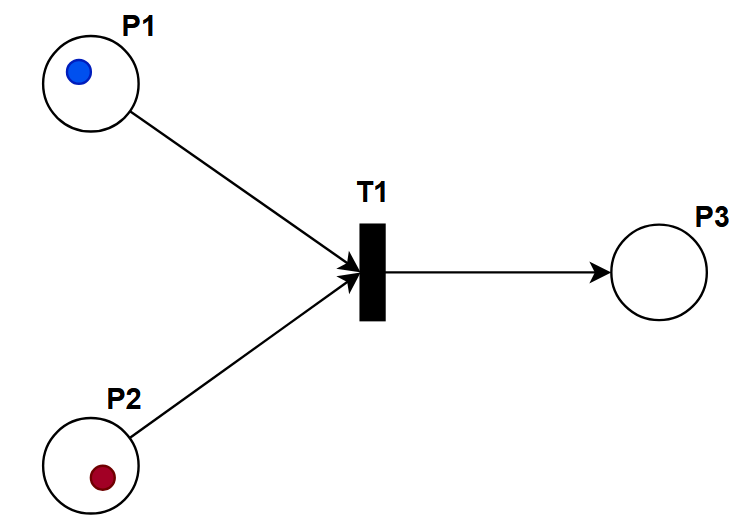
\includegraphics[width=\textwidth]{imgs/Cap2_teoria/CPN1.png}
		\caption{Before firing $T_1$}
		\label{fig:cpn1}
	\end{subfigure}
	\hfill
	\begin{subfigure}[b]{0.48\textwidth}
		\centering
		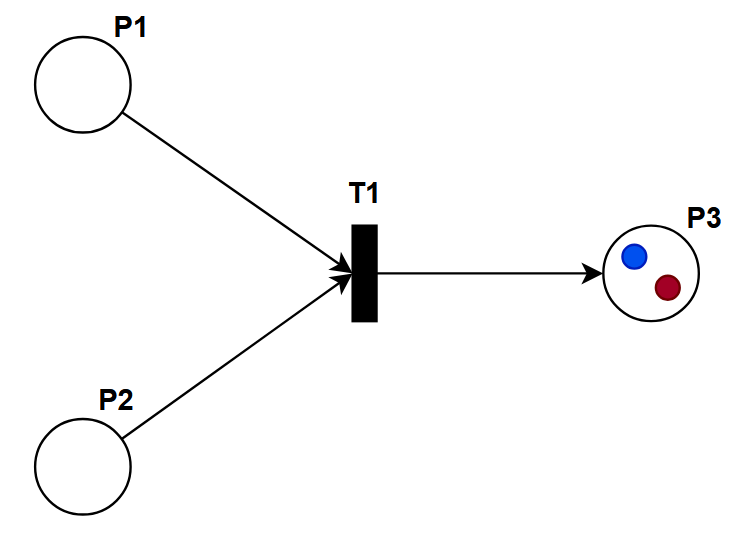
\includegraphics[width=\textwidth]{imgs/Cap2_teoria/CPN3.png}
		\caption{After firing $T_1$}
		\label{fig:cpn2}
	\end{subfigure}
	
	\caption{Example of transition firing in a Colored Petri Net.}
	\label{fig:cpn}
\end{figure}

\noindent Initially, the colored markings of the individual places are

\[
M_0(P_1)=
\begin{bmatrix}
	1 & 0
\end{bmatrix}^{\mathsf T},
\qquad
M_0(P_2)=
\begin{bmatrix}
	0 & 1
\end{bmatrix}^{\mathsf T},
\qquad
M_0(P_3)=
\begin{bmatrix}
	0 & 0
\end{bmatrix}^{\mathsf T}.
\]

\noindent Considering the component order

\[
(P_1^{b},P_1^{r},
P_2^{b},P_2^{r},
P_3^{b},P_3^{r}),
\]

\noindent the global colored marking can equivalently be written as

\[
M_0=
\begin{bmatrix}
	1 & 0 & 0 & 1 & 0 & 0
\end{bmatrix}^{\mathsf T}.
\]

\noindent Since transition $T_1$ consumes one blue token from $P_1$ and one red token from $P_2$, while producing both tokens in $P_3$, the corresponding colored incidence vector is

\[
C_{T_1}
=
\begin{bmatrix}
	-1 & 0 & 0 & -1 & 1 & 1
\end{bmatrix}^{\mathsf T}.
\]

\noindent The new marking after the firing of $T_1$ is obtained through the marking equation

\[
M_1=M_0+C_{T_1},
\]

\noindent hence

\[
M_1=
\begin{bmatrix}
	1\\
	0\\
	0\\
	1\\
	0\\
	0
\end{bmatrix}
+
\begin{bmatrix}
	-1\\
	0\\
	0\\
	-1\\
	1\\
	1
\end{bmatrix}
=
\begin{bmatrix}
	0\\
	0\\
	0\\
	0\\
	1\\
	1
\end{bmatrix}.
\]

\noindent Therefore, after the firing of $T_1$, both input places are empty, while $P_3$ contains one blue token and one red token.

\subsection{Colored Timed Petri Nets and persistent state}
\label{sec:theory-ctpn}

A Colored Timed Petri Net (CTPN) adds timing information to the colored
state representation. In the warehouse model, a mission that starts at
$s_m$ and has simulated duration $\tau_m$ completes at $c_m=s_m+\tau_m$.
The marking and token colors encode precedence and resource ownership,
while the temporal mechanism represents concurrent execution.

The assignment decision belongs to the scheduler. Once an order receives
a resource, the net preserves that resource's token along the sequence of
missions, returning it to the common resource place only at the end of the
order. The preceding single-mission release examples describe the general
formalism; the order-level design extends the reservation across intermediate
missions. A scheduling batch is a group of admitted work, not a reset of the
net: its end preserves the marking and any unfinished order on its owner.


\section{Scheduling basics}
\label{sec:scheduling-basics}

Scheduling determines which resource performs each activity and when that
activity can start. In a warehouse, these decisions must account for resource
compatibility, the work already assigned, and dependencies between missions.
The resulting schedule can then be evaluated through completion times, workload
distribution, and respect for due dates.

In this thesis, assignment is made at the level of an \textit{order}. Each order
contains several missions, which must all retain the same assigned resource.
Resources can work in parallel, but each resource executes at most one mission
at a time. The following concepts provide the basis for the scheduler described
in the next chapter.

\subsection{Resource compatibility and order assignment}
\label{sec:theory-eligibility}

A resource is \textit{eligible} for a mission if it meets the requirements needed
to execute it. For example, a mission may require a particular type of forklift.
Scheduling problems with these restrictions are reviewed
in~\cite{leung2008processing,leung2016processing}. Compatibility does not imply
immediate availability: a suitable resource may still be busy with another task.
Both aspects are considered in~\cite{liao2008parallel}, although that study uses
different execution assumptions from the warehouse model considered here.

Let $\mathcal O$ be the set of orders, $\mathcal R$ the set of resources, and
$\mathcal M_o^{\mathrm{adm}}$ the missions of order $o$ retained after data
preparation. If $\mathcal R_m$ is the set of resources eligible for mission $m$,
the resources eligible for the whole order are
\begin{equation}
    \mathcal R_o=\bigcap_{m\in\mathcal M_o^{\mathrm{adm}}}\mathcal R_m.
    \label{eq:order-eligible-resources}
\end{equation}
This intersection selects only resources capable of performing every retained
mission of the order. For example, if one mission can use resources 1 and 2,
and another can use resources 2 and 3, the order must be assigned to resource 2.
If there is no common resource, the order cannot be assigned under these rules.

Each order admitted to execution receives exactly one eligible resource.
Writing $x_{or}=1$ when order $o$ is assigned to resource $r$, and zero otherwise,
this condition becomes
\begin{equation}
    \sum_{r\in\mathcal R_o}x_{or}=1,
    \qquad\text{for each order admitted to execution},
    \label{eq:unique-order-assignment}
\end{equation}
with $x_{or}=0$ for ineligible resources. The selected resource becomes the
order's \textit{owner} when its first mission enters a queue. Later missions
retain that owner, even if they are admitted in different batches. Thus, keeping
an order on one resource does not require placing all its missions in the same
batch.

\subsection{List scheduling and load balancing}
\label{sec:theory-list-scheduling}

A simple way to build a schedule is to consider activities in a priority list
and assign them progressively. In \textit{list scheduling}, an available
resource receives the next activity that can start according to the list;
any required predecessors must already be complete~\cite{graham1966bounds}.
A \textit{greedy} rule makes each decision using the current alternatives,
without comparing all possible future schedules.

One common rule assigns the next activity to the least-loaded resource.
For independent activities on identical resources, let $\mathcal A_r$ contain
the activities already assigned to resource $r$, and let $\tau_j$ be the
processing time of activity $j$. The assigned load is
\begin{equation}
    L_r=\sum_{j\in\mathcal A_r}\tau_j.
    \label{eq:theory-assigned-load}
\end{equation}
For example, if two eligible resources have 30 and 50 minutes of assigned work,
a new activity lasting 10 minutes is assigned to the first. Their loads become
40 and 50 minutes. This illustrates load balancing by processing time rather
than by number of activities.

With compatibility restrictions, the choice is limited to eligible resources.
If an activity takes different amounts of time on different resources, the
rule can compare the resulting loads $L_r+\tau_{jr}$, where $\tau_{jr}$ is its
processing time on resource $r$. In the warehouse, this reasoning must also
respect order ownership and mission dependencies.

A greedy decision does not guarantee the best complete schedule. Proven
performance guarantees, such as those studied in~\cite{4568274}, apply to
specific algorithms and assumptions; they cannot be transferred directly to
the warehouse heuristic.

\subsection{Progressive decisions, queues and batches}
\label{sec:theory-batch-queues}

In \textit{offline} scheduling, the activities are known in advance. In
\textit{online} scheduling, new activities or information become available
during execution. Online load balancing with irrevocable assignments is
studied in~\cite{aspnes1997online}. In this thesis, the orders are known at the
start, but assignment decisions are made progressively as execution unfolds.
Making decisions during execution does not, by itself, make the problem online.

A resource queue holds work admitted for that resource and not yet completed.
\textit{Admission} determines which missions enter the queue;
\textit{dispatching} determines which admitted mission starts when the required
conditions are satisfied. A batch groups missions admitted at a scheduling
step. Smaller batches allow more frequent decisions, while larger batches
commit more work in advance.

Queue length and workload measure different things. A queue containing two
long missions can require more time than one containing five short missions.
For a queue $\mathcal Q_r(t)$ at time $t$,
\begin{equation}
    N_r^{\mathrm q}(t)=|\mathcal Q_r(t)|,
    \qquad
    \widehat L_r^{\mathrm q}(t)=
        \sum_{j\in\mathcal Q_r(t)}\widehat\tau_{jr},
    \label{eq:queue-estimated-workload}
\end{equation}
where $N_r^{\mathrm q}(t)$ counts the queued activities and
$\widehat\tau_{jr}$ estimates the processing time still required by each one.
Balancing queue lengths therefore need not balance execution times.

\subsection{Execution times and due dates}
\label{sec:theory-deadlines}

A mission is \textit{non-preemptive} if, once started, it runs to completion
without interruption. This does not prevent an order from waiting between two
successive missions. In this thesis, retaining the same owner throughout an
order is an additional assignment constraint.

For an activity $j$, the release time $r_j$ is the earliest time at which it
becomes available, $S_j$ is its actual start, and $C_j$ is its completion.
With processing time $\tau_j$,
\[
    S_j\geq r_j,\qquad C_j=S_j+\tau_j.
\]
Activities cannot overlap on the same resource. If one activity must precede
another, it must also finish before the next one starts.
The total time from release to completion is called \textit{flow time}:
\begin{equation}
    F_j=C_j-r_j.
    \label{eq:order-flow-time}
\end{equation}
It includes both waiting and processing. For an order containing several
missions, completion refers to the end of its final mission, so the elapsed
time can also include waits between missions.

Before execution, processing times may be estimated rather than known exactly.
An estimate $\widehat\tau_j$ represents the expected work, whereas a
\textit{due date} $d_j$ specifies the target completion time. Travel, resource
choice and execution sequence can affect the estimate; waiting for resources
can further delay completion.

When a target is defined by a time allowance $b_j$, its reference instant
$a_j$ must be specified:
\begin{equation}
    d_j=a_j+b_j.
    \label{eq:relative-deadline-scheduling}
\end{equation}
For example, a two-hour allowance measured from release includes the initial
waiting time; the same allowance measured from actual start excludes it.
Updating a completion-time estimate does not automatically change the due date.
A due date may be a soft target, whose violation is measured, or a hard deadline
that a feasible schedule must meet.

\subsection{Delay and time margin}

For an order $o$ completed at time $C_o$ with due date $d_o$, \textit{lateness}
measures the signed difference between completion and target:
\begin{equation}
    L_o=C_o-d_o.
    \label{eq:order-lateness}
\end{equation}
A negative value means early completion; a positive value means late completion.
\textit{Tardiness} counts only positive delay:
\begin{equation}
    T_o=\max\{0,C_o-d_o\}.
    \label{eq:order-tardiness}
\end{equation}
An order completed ten minutes early therefore has lateness of $-10$ minutes
and zero tardiness. The completion margin expresses the same result with the
opposite sign:
\begin{equation}
    \sigma_o=d_o-C_o=-L_o.
    \label{eq:order-slack}
\end{equation}
A positive margin means that time remained before the due date at completion.

For an unfinished order, \textit{slack} instead estimates the time available
beyond the work still required. At time $t$,
\[
    s_o(t)=d_o-t-\widehat\tau_o^{\mathrm{rem}}(t),
\]
where $\widehat\tau_o^{\mathrm{rem}}(t)$ is the estimated remaining processing
time. If the due date is 30 minutes away and 20 minutes of work remain, the
slack is 10 minutes. Further waiting may consume this margin, so positive slack
does not guarantee timely completion.

\subsection{Makespan and resource utilization}

The \textit{makespan} is the time at which the last activity finishes,
measured from the chosen time origin. For the set of activities $\mathcal J$,
\begin{equation}
    C_{\max}=\max_{j\in\mathcal J}C_j.
    \label{eq:makespan-basic}
\end{equation}
Reducing makespan means completing the whole workload sooner. This is a common
objective in parallel-resource scheduling~\cite{leung2016processing}.

Due-date performance can instead be measured by the number of late orders,
\begin{equation}
    N_{\mathrm{late}}=\sum_{o\in\mathcal O}U_o,
    \qquad
    U_o=\begin{cases}1,&C_o>d_o,\\0,&C_o\leq d_o,\end{cases}
    \label{eq:number-late-orders}
\end{equation}
or by total and maximum tardiness:
\begin{equation}
    T_{\mathrm{tot}}=\sum_{o\in\mathcal O}T_o,
    \qquad T_{\max}=\max_{o\in\mathcal O}T_o.
    \label{eq:tardiness-indicators}
\end{equation}
These indicators answer different questions: how many orders are late, how
much delay accumulates, and how severe the worst delay is. If execution is
incomplete, completed orders must be evaluated separately from unfinished work.

The processing workload of resource $r$ is the sum of the durations of its
assigned activities:
\begin{equation}
    W_r=\sum_{j\in\mathcal A_r}\tau_{jr}.
    \label{eq:actual-resource-workload}
\end{equation}
This excludes idle time. A resource with six hours of work may finish later
than hour six if it must wait between activities. Consequently, the largest
workload equals makespan only when execution starts at time zero and proceeds
without idle gaps or additional setup time.

Resource utilization is the fraction of an observation interval spent working.
For an interval of duration $H$, if resource $r$ is busy for $B_r$ time units,
its utilization is $U_r=B_r/H$ and its idle time is $H-B_r$. For example,
six busy hours in an eight-hour interval give a utilization of $75\%$.
Resources must be compared over the same observation interval. Workload balance,
utilization, makespan and delays describe different aspects of performance;
improving one does not necessarily improve the others.



\chapter{Proposed approach}
The following chapter describes the design behind the assignment of the missions to the resources. The system considers \textit{eight} resources, each of one is the composition of human operator and forklift. The orders are known at the beginning of the startup and they are assigned progressively, keeping every mission of a singular order attached to their resource.

The 

La politica organizza le decisioni mediante interventi globali di batching.
Il parametro $x$ definisce il
numero di nuove missioni da aggiungere a ogni refill e, nella configurazione
adottata, il numero di completamenti globali che attiva l'intervento
successivo. Le nuove missioni si aggiungono al lavoro eventualmente residuo:
$x$ non costituisce una capienza massima dell'insieme delle missioni ammesse.

La simulazione conserva lo stato delle risorse durante ciascuna
riassegnazione. Una risorsa con una missione in esecuzione mantiene il
percorso e il completamento programmato; una risorsa che ha esaurito la
propria coda può ricevere nuovo lavoro a partire dall'istante in cui l'ha
terminata. L'istante della decisione globale viene pertanto distinto dagli
istanti locali di inserimento delle nuove missioni. Il metodo costruisce
una pianificazione offline, nella quale è possibile completare
retroattivamente la timeline delle singole risorse.

L'esecuzione è governata da Colored Timed Petri Net (CTPN), che rappresenta le precedenze e la
riserva della risorsa. Il planner A* determina percorsi e durate delle
missioni avviate. La stima euclidea è utilizzata esclusivamente per fissare
le deadline degli ordini e valutarne il rispetto a posteriori; non
interviene nell'assegnazione, nel refill o nell'abilitazione degli avvii.

Nel modello discusso si assume che i dati preparati definiscano missioni
eseguibili e che tutte le missioni ammesse vengano portate a termine. 

\section{Ordini, missioni e risorse}
\label{sec:progetto-modello}

Siano $\mathcal O=\{o_1,\ldots,o_N\}$ l'insieme degli ordini e
$\mathcal R=\{1,\ldots,R\}$ quello delle risorse, con $R=8$ nella
configurazione di riferimento. Ogni ordine $o$ comprende un insieme di
missioni $\mathcal M_o$, di cardinalità $n_o=|\mathcal M_o|$.
Una missione descrive una movimentazione da un punto di prelievo FROM a un
punto di destinazione TO ed è caratterizzata da un codice, una priorità e
un'associazione all'ordine.

Ogni riga del dataset riceve anche un identificativo univoco di occorrenza.
Due missioni con lo stesso codice commerciale rimangono quindi attività
distinte. Una missione priva di identificativo d'ordine viene trattata come
un ordine autonomo, senza accorpare tra loro tutte le righe prive di tale
informazione.

Si indica con $\mathcal M_o^{\mathrm{adm}}$ l'insieme delle missioni
dell'ordine considerate dopo la preparazione dei dati. Il completamento
descritto nel seguito è riferito a tale insieme. La preparazione verifica
le informazioni necessarie e normalizza le coordinate prima
dell'assegnazione; le eventuali righe non ammesse rimangono esterne alla
rete operativa.

\begin{nota}
	Uno script Python divide i dati aziendali per giorno lavorativo. Ogni
	ordine resta interamente nello stesso lotto. Gli ordini del giorno sono
	noti prima di avviare la simulazione.
\end{nota}

\subsection{Vincolo di assegnazione ordine--risorsa}

Indicando con $r(o)$ la risorsa proprietaria dell'ordine, si impone
\begin{equation}
	r(m)=r(o),\qquad \forall m\in\mathcal M_o^{\mathrm{adm}}.
\end{equation}
Il proprietario viene scelto quando la prima missione dell'ordine viene
accodata. L'associazione resta invariata anche quando l'ordine attraversa
più interventi di batching. L'indivisibilità riguarda l'assegnazione alla
risorsa: non impone di inserire tutte le missioni dell'ordine in un unico
blocco di ammissione.

Una risorsa può essere proprietaria di più ordini, ma ne esegue uno alla
volta. Dall'avvio di un ordine fino alla conclusione della sua sequenza,
il token rimane riservato a quell'ordine. Le sue missioni non vengono
intercalate con quelle di altri ordini.

\subsection{Priorità e precedenze interne}

A ogni missione $m$ è associata una priorità numerica $p_m$. La sequenza
interna dell'ordine è
\begin{equation}
	\pi_o=(m_{o,1},\ldots,m_{o,n_o^{\mathrm{adm}}}),\qquad
	p_{m_{o,i}}\geq p_{m_{o,i+1}},
\end{equation}
dove $n_o^{\mathrm{adm}}=|\mathcal M_o^{\mathrm{adm}}|$.
A parità di priorità si mantiene l'ordine di ingresso; una priorità
mancante assume il valore convenzionale unitario.

Questa regola riguarda soltanto le missioni dello stesso ordine. I nuovi
ordini compatibili vengono considerati secondo la loro prima comparsa nel
dataset, senza ordinamenti per numero di missioni, durata prevista,
distanza o deadline. Le missioni residue di ordini già assegnati alla
risorsa hanno precedenza sull'apertura di nuovi ordini.

\section{Politica di assegnazione ordini}
\label{sec:progetto-assegnazione}

La politica applica i vincoli di compatibilità e assegnazione univoca
introdotti nella Sezione~\ref{sec:theory-eligibility}. Distingue
l'ammissione di nuovo lavoro dal dispatching delle missioni già in coda,
secondo la Sezione~\ref{sec:theory-batch-queues}. Lo scheduler stabilisce
quali attività aggiungere mentre la CTPN stabilisce quando tali attività possono
iniziare.

\subsection{Compatibilità dell'intero ordine}

Sia $\mathcal R_m\subseteq\mathcal R$ l'insieme delle risorse compatibili
con la missione $m$. Per l'ordine si considera
\begin{equation}
	\mathcal R_o=\bigcap_{m\in\mathcal M_o^{\mathrm{adm}}}\mathcal R_m.
\end{equation}
Per il problema corrente assume $\mathcal R_o\neq\varnothing$ per ogni
ordine. Il proprietario viene scelto in questo insieme, garantendo che
possa eseguire l'intera sequenza. L'associazione viene fissata dalla prima ammissione e
conservata nei refill successivi.

\subsection{Blocco globale e refill additivo}

Sia $k$ l'indice dell'intervento di batching. Si distinguono:
\begin{itemize}
	\item $\mathcal A_k^{-}$, le missioni già ammesse e non ancora
	completate prima del refill, comprendenti attese ed esecuzioni;
	\item $\mathcal N_k$, le nuove missioni inserite durante il refill;
	\item $\mathcal A_k^{+}$, il lavoro ammesso dopo l'assegnazione.
\end{itemize}
Le missioni nuove sono distinte dai residui e valgono
\begin{equation}
	\mathcal A_k^{+}=\mathcal A_k^{-}\cup\mathcal N_k,
	\qquad \mathcal A_k^{-}\cap\mathcal N_k=\varnothing,
	\label{eq:refill-insiemi}
\end{equation}
\begin{equation}
	|\mathcal N_k|\leq x,\qquad
	|\mathcal A_k^{+}|=|\mathcal A_k^{-}|+|\mathcal N_k|.
	\label{eq:refill-additivo}
\end{equation}
Quando rimangono almeno $x$ missioni assegnabili, $|\mathcal N_k|=x$, queste verranno inserite nell'ultimo blocco di rifornimento per le risorse.
Le $x$ missioni costituiscono il totale globale da distribuire tra le
risorse, non una quantità assegnata a ciascuna risorsa. Il lavoro residuo non riduce la dimensione del nuovo blocco. 
\begin{example}[Mission admission set]
	Con sette missioni ancora ammesse e $x=20$, un refill completo porta il
	lavoro ammesso a ventisette missioni. L'ammissione non si basa su un numero
	di posti liberi rispetto a una capienza fissa.
\end{example}

Si indica con $C_k$ il numero di eventi di completamento registrati nel
passaggio di esecuzione successivo all'assegnazione $k$ mentre il contatore delle missioni completate viene
azzerato all'inizio del passaggio. Al raggiungimento di
\begin{equation}
	C_k=x
	\label{eq:trigger-refill}
\end{equation}
il motore sospende l'elaborazione prima di ulteriori avvii e, se rimane
lavoro da assegnare, richiama lo scheduler. L'esaurimento della coda di una sola risorsa
non attiva autonomamente un refill.

Il contatore riguarda i completamenti elaborati nel passaggio, anche
quando appartengono a missioni ammesse in precedenza. Non va identificato
con un conteggio effettuato soltanto tra due istanti globali della timeline
finale, poiché nuovi eventi possono essere inseriti retroattivamente.

\begin{nota}
	Con inizializzazione vuota, primo blocco di $x$ missioni e soglia pari a
	$x$ completamenti, il primo refill avviene quando quel blocco è interamente
	concluso. La conservazione del lavoro residuo è una proprietà della
	procedura, non implica che a ogni confine vi siano necessariamente
	missioni in esecuzione. A parità di blocco e soglia, in assenza di residui
	iniziali, questa stessa condizione si ripete nei passaggi successivi.
\end{nota}

\subsection{Distribuzione delle missioni tra le risorse}

I principi di list scheduling della
Sezione~\ref{sec:theory-list-scheduling} vengono applicati considerando il
numero di missioni già ammesse per ciascuna risorsa. Per ogni risorsa si
definisce
\begin{equation}
	q_r=|\{m\in\mathcal A:\ r(m)=r\}|,
\end{equation}
dove $\mathcal A$ è l'insieme delle missioni ammesse ma non ancora
completate. Il conteggio include quindi sia la missione eventualmente in
esecuzione sia quelle presenti in coda.

Le risorse vengono considerate a partire da quella con il valore di $q_r$
più basso, così da favorire quelle che hanno meno missioni già assegnate.
In caso di parità, viene data precedenza alla risorsa che dispone di meno
ordini compatibili ancora non assegnati. Se una risorsa possiede già un
ordine con missioni ancora da accodare, tale condizione le conferisce
priorità. Gli eventuali ulteriori pareggi sono risolti in base all'indice
della risorsa. Il numero di ordini compatibili viene determinato all'inizio
dell'intervento, mentre $q_r$ viene aggiornato dopo ogni nuova ammissione.

Una volta scelta la risorsa, la missione da ammettere viene individuata
secondo due regole:
\begin{enumerate}
	\item Se esistono missioni ancora pendenti appartenenti a un ordine già
	assegnato alla risorsa, viene scelta la prima disponibile, nel rispetto
	delle precedenze interne all'ordine;
	\item In assenza di missioni proprie da accodare, viene selezionato il
	primo ordine compatibile ancora non assegnato, secondo l'ordine di
	ingresso, e ne viene ammessa la prima missione pendente.
\end{enumerate}
Dopo ogni inserimento il valore di $q_r$ viene aggiornato e la procedura
prosegue fino al completamento del nuovo blocco o all'esaurimento del
lavoro disponibile. Le missioni già presenti in coda mantengono comunque
la precedenza rispetto a quelle aggiunte successivamente.

Il criterio mira quindi a distribuire tra le risorse il numero di missioni
ammesse, senza utilizzare una stima della loro durata. Di conseguenza, non
garantisce né carichi temporali uguali né che tutte le risorse rimangano
continuamente occupate. Il tempo di lavoro effettivo dipende infatti dai
percorsi delle missioni e dalle caratteristiche degli ordini assegnati.

\subsection{Riferimento temporale nominale}

Il tempo nominale per missione $\overline{\tau}=180\,\mathrm{s}$ consente
di definire il riferimento
\begin{equation}
	H=\frac{x\,\overline{\tau}}{R}.
	\label{eq:budget_temporale_batch}
\end{equation}
Indicando con $T_k$ l'istante della decisione globale $k$, si associa al
passaggio la scadenza nominale
\begin{equation}
	D_k=T_k+H.
\end{equation}
Questo riferimento è utilizzato soltanto nel report. Non dimensiona le
code, non determina il refill e non interrompe l'esecuzione. La durata
delle missioni viene ricavata da A*. \begin{comment}
	mentre le deadline dei singoli ordini
	seguono il modello euclideo della
	Sezione~\ref{sec:stima-deadline-euclidea}.
\end{comment}


\section{CTPN per la riserva della risorsa}
\label{sec:progetto-ctpn}

Il modello applica la rappresentazione colorata temporizzata introdotta
nella Sezione~\ref{sec:theory-ctpn}, specializzando la riserva del token
alla sequenza di missioni di un ordine.

\begin{figure}[H]
	\centering
	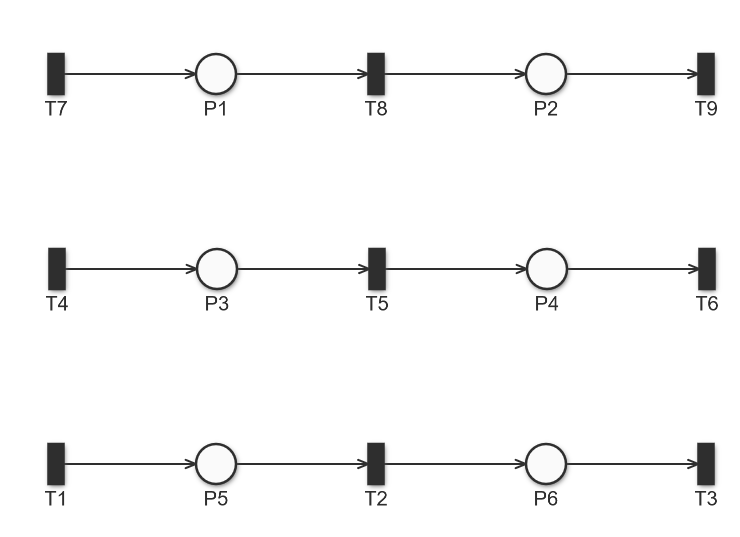
\includegraphics[width=0.7\linewidth]{imgs/Cap2_teoria/NEW_PN2_VECCHIA_MISSIONI}
	\caption{Schema di riferimento della modellazione precedente delle alternative di risorsa per una singola missione.}
	\label{fig:pn2vecchiamissioni}
\end{figure}


\noindent La Figura~\ref{fig:pn2vecchiamissioni} richiama lo schema precedente,
organizzato intorno alle alternative di risorsa per una singola missione.
Nella soluzione adottata lo scheduler assegna la risorsa all'intero ordine
quando accoda la prima missione. La rete
non seleziona un nuovo proprietario
per ogni missione, ma utilizza il colore della risorsa già assegnata.


Ciascuna missione mantiene una sottorete con tre transizioni e due posti
interni. Le tre fasi rappresentano l'avvio, il completamento temporizzato
e il passaggio alla missione seguente oppure il rilascio della risorsa.
Le sottoreti dello stesso ordine vengono collegate in sequenza secondo
le priorità interne.

\subsection{Intra-order links}
Tra due missioni consecutive viene inserito un posto di collegamento che
riceve il token dalla transizione finale della precedente e lo rende
disponibile alla transizione iniziale della successiva. Il token conserva
il colore della risorsa assegnata. Il posto di collegamento rappresenta
quindi sia la precedenza sia il mantenimento della riserva operativa.

La Figura~\ref{fig:pn1nuovamissioni} mostra una sequenza di tre missioni;
i posti $P7$ e $P8$ collegano le rispettive sottoreti. Lo schema evidenzia
le precedenze e va letto insieme al vincolo sul colore della risorsa.

\begin{figure}[H]
	\centering
	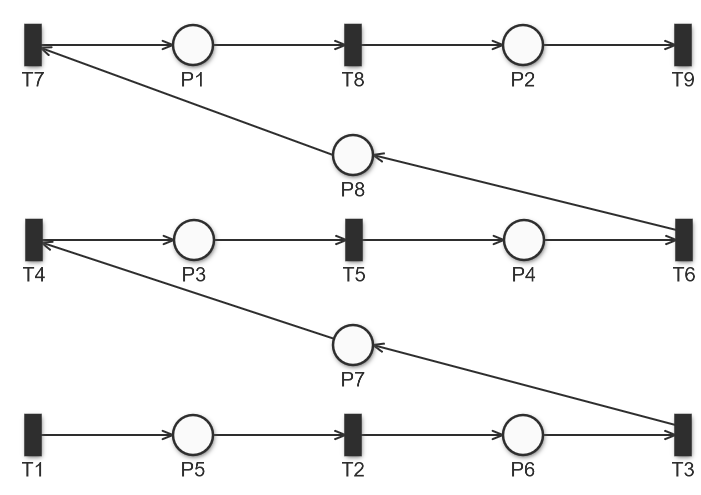
\includegraphics[width=0.7\linewidth]{imgs/Cap2_teoria/NEW_PN1_NUOVA_MISSIONI}
	\caption{Collegamento tra tre missioni dello stesso ordine mediante posti di precedenza. Il token della risorsa viene trasferito lungo la sequenza senza essere restituito al posto comune tra missioni intermedie.}
	\label{fig:pn1nuovamissioni}
\end{figure}

Solo la prima missione dell'ordine preleva il token dal posto comune delle
risorse disponibili; solo l'ultima missione ammessa lo restituisce.
All'interno dell'ordine, la disponibilità necessaria all'avvio è rappresentata
dal token nel posto di collegamento: non occorre prelevare nuovamente una
risorsa libera dal posto comune.

Per ogni risorsa $r\in\mathcal R$ esiste esattamente un token di colore
$r$ nella rete operativa. La conservazione del token è espressa
dall'invariante di posto
\begin{equation}
	\sum_{p\in\mathcal P}M(p)(r)=1,
	\qquad \forall r\in\mathcal R,
\end{equation}
dove $M(p)(r)$ indica la molteplicità del colore $r$ nel posto $p$ e
$\mathcal P$ è l'insieme dei posti della rete. La marcatura determina le
transizioni abilitate, mentre l'associazione ordine--risorsa stabilisce
il colore che può partecipare al loro scatto.

\begin{nota}
	Per semplicità di rappresentazione, le reti di Petri mostrate nelle figure non sono CPN, bensì PN. Questo perché ciascuna figura rappresenta un singolo ramo della rete, percorso da token appartenenti a un unico colore, consentendo così una rappresentazione grafica semplificata.
\end{nota}

\subsection{Conservazione della riserva durante il refill}

La sospensione per il batching non costituisce una transizione di rilascio.
Il token di una risorsa in esecuzione rimane nel posto di lavoro della
missione corrente. Anche il token che attende la missione successiva dello
stesso ordine rimane nel posto di collegamento, senza tornare al posto
comune. La risorsa viene rilasciata soltanto alla conclusione dell'ordine.

Il refill modifica le ammissioni e, per i nuovi ordini, l'associazione alla
risorsa. Non ricostruisce la rete, non reinizializza la marcatura e non
ricalcola il percorso di una missione già avviata. L'avvio richiede
congiuntamente l'ammissione della missione e l'abilitazione della relativa
transizione nella CTPN.

\section{Continuità dello stato tra batch}
\label{sec:progetto-tempo}

\subsection{Stato persistente e risorse in esecuzione}

Tra due interventi si conservano la \textbf{marcatura}, i \textbf{proprietari degli ordini},
le \textbf{code residue}, le \textbf{posizioni raggiunte}, i \textbf{percorsi delle missioni avviate}
e i \textbf{relativi istanti di inizio} e \textbf{fine programmata}. Vengono conservati anche
la cronologia dei completamenti e i valori delle deadline già fissate.
Il contatore $C_k$ viene invece azzerato per il nuovo passaggio.

L'indicatore \textit{in work} rappresenta il numero di risorse con una
missione avviata e non ancora completata nello stato sospeso. Non comprende
le missioni soltanto in attesa. Poiché ogni risorsa può eseguire una sola
missione alla volta, tale indicatore coincide con il numero di missioni
attualmente in esecuzione.

\subsection{Eventi di esecuzione e soglia globale}

L'avanzamento riprende il principio della Scheduled Event List descritto
nella Sezione~\ref{sec:theory-sel}. Per una missione $m$ avviata
all'istante $s_m$ e di durata $\tau_m$, il completamento è programmato a
\begin{equation}
	c_m=s_m+\tau_m.
\end{equation}
Il motore elabora gli eventi concorrenti e incrementa $C_k$ a ogni
completamento. Finché la soglia non è raggiunta, una risorsa può avviare la
successiva missione ammessa e abilitata, senza richiamare lo scheduler.

Quando $C_k=x$, il motore conserva lo stato prima di altri avvii. Gli altri
eventi eventualmente programmati allo stesso istante vengono elaborati
nel passaggio successivo, senza introdurre un ritardo fisico. Questa
convenzione mantiene esatto il conteggio dei completamenti del passaggio.

Se non rimangono nuove missioni da ammettere, il motore continua a eseguire
il lavoro già assegnato. La simulazione termina quando tutte le missioni
ammesse dopo la preparazione sono completate. L'ultimo passaggio può
contenere meno di $x$ completamenti quando il lavoro residuo è inferiore
alla soglia.

\subsection{Decisione globale e ripartenza locale}

Si distingue l'istante $T_k$ della decisione globale dal cursore temporale
$\theta$ usato per elaborare gli eventi. Le decisioni globali mantengono
una sequenza non decrescente; il cursore può invece tornare a un istante
precedente per inserire lavoro sulla timeline di una risorsa.

Per una risorsa che ha esaurito la propria coda, sia $f_{r,k}$ il suo ultimo
istante di completamento noto prima del refill. Il nuovo lavoro può essere
inserito a partire da
\begin{equation}
	a_{r,k}=f_{r,k},
	\label{eq:ripartenza-locale}
\end{equation}
anche quando $a_{r,k}<T_k$. Per una risorsa mai impiegata, la frontiera
iniziale è posta a zero. Se la risorsa conserva lavoro in coda o in
esecuzione, le aggiunte rispettano tale lavoro e non ne anticipano
l'esecuzione.


\begin{example}[Back-to-the-Future assignment]
	Una risorsa che ha terminato la coda a $80\,\mathrm{s}$ può
	ricevere il blocco successivo a partire da tale istante anche se la
	decisione globale viene registrata a $120\,\mathrm{s}$. Il nuovo lavoro
	viene inserito nell'intervallo temporale precedentemente rimasto libero.
\end{example}

\noindent Il ritorno temporale non annulla gli eventi già consolidati sulle altre
risorse. Ciascuna mantiene la propria frontiera: non si avviano due
missioni contemporaneamente sulla stessa risorsa e non si modifica una
missione già in work. In particolare, il suo istante di completamento
$c_m$ rimane quello definito all'avvio.

Gli eventi aggiunti nel passato appartengono al nuovo passaggio di
elaborazione. Se il cursore raggiunge il target in un istante
$\theta_k^{\mathrm{stop}}$ precedente all'ultima decisione globale,
l'istante della decisione seguente è registrato come
\begin{equation}
	T_{k+1}=\max\{T_k,\theta_k^{\mathrm{stop}}\}.
	\label{eq:decisione-globale}
\end{equation}
Questa distinzione evita di attribuire a tutte le risorse un unico istante
di ripartenza e separa la sequenza delle decisioni dalla timeline finale.

\begin{nota}
	La procedura costruisce una pianificazione offline a partire da ordini
	noti. L'inserimento retroattivo completa la timeline simulata; non descrive
	un comando che un sistema fisico potrebbe eseguire nel passato. Le durate
	di calcolo del programma non vengono sommate ai tempi operativi simulati.
\end{nota}



\begin{comment}
	
	\subsection{Procedura di batching}
	
	La sequenza operativa può essere riassunta nei seguenti passi:
	\begin{enumerate}
		\item conservare tutte le missioni ammesse non ancora completate e lo
		stato delle risorse;
		\item aggiungere fino a $x$ nuove missioni, privilegiando le continuazioni
		degli ordini già assegnati e mantenendo l'ingresso per i nuovi ordini;
		\item per le risorse con coda esaurita, riprendere dalla rispettiva
		frontiera temporale; mantenere le esecuzioni delle altre risorse;
		\item elaborare le missioni ammesse tramite la CTPN e i percorsi A*,
		contando globalmente i completamenti;
		\item alla soglia $x$, sospendere l'elaborazione, registrare lo stato e
		ripetere il procedimento; terminare quando tutto il lavoro è concluso.
	\end{enumerate}
	
	
\end{comment}


\section{Stima euclidea delle deadline}
\label{sec:stima-deadline-euclidea}
\label{sec:stima-deadline-manhattan} % Alias per i riferimenti preesistenti.

Le scadenze applicano le definizioni della
Sezione~\ref{sec:theory-deadlines}. Sono indicatori osservativi, calcolati
per confrontare la previsione geometrica con i tempi di completamento.
Non vengono utilizzate per scegliere ordini, dimensionare code, assegnare
risorse o attivare refill.

La deadline dell'ordine viene fissata al primo avvio effettivo di una sua
missione. Non decorre dall'assegnazione del proprietario: l'attesa dovuta
agli ordini precedenti non consuma il budget del nuovo ordine. Tutte le
scadenze cumulative dell'ordine vengono congelate insieme e non vengono
ricalcolate durante i refill o la ripresa delle missioni successive.

\subsection{Sequenza e distanza stimata}

Si considera la sequenza $\pi_o$ delle missioni ammesse dell'ordine,
ordinata secondo le precedenze interne. Gli estremi $F_i$ e $T_i$ sono gli
indici della griglia corrispondenti a FROM e TO dopo normalizzazione e
arrotondamento. La previsione usa
\begin{equation}
	d_E(p,q)=\sqrt{(x_p-x_q)^2+(y_p-y_q)^2}.
	\label{eq:manhattan-distance} % Nome storico mantenuto per compatibilita.
\end{equation}
Sia $P_r$ la posizione della risorsa prima del primo avvio dell'ordine.
Si pone $Q_1=P_r$ e $Q_i=T_{i-1}$ per $i>1$; quando la risorsa non ha una
posizione precedente, si assume $Q_1=F_1$. La distanza prevista per ciascuna
missione è
\begin{equation}
	\widehat\ell_{o,i}=d_E(Q_i,F_i)+d_E(F_i,T_i).
	\label{eq:estimated-order-distance}
\end{equation}
Si includono così l'avvicinamento iniziale e gli spostamenti tra le
missioni consecutive. La previsione non esegue A* e non applica le
correzioni verso celle libere e raggiungibili effettuate dal planner.\footnote{La distanza euclidea è calcolata con la stessa formula utilizzata
	per stimare il tempo medio di percorrenza nell'algoritmo A*.}

Con velocità $v_c=5.5$ celle al secondo, maggiorazione $\alpha=0.20$,
contributo accessorio $\tau_f=60\,\mathrm{s}$ e margine
$\delta_m=30\,\mathrm{s}$ per missione, la durata prevista è
\begin{equation}
	\widehat\tau_{o,i}=
	\operatorname{round}\!\left(
	\frac{\widehat\ell_{o,i}}{v_c}(1+\alpha)\right)
	+\tau_f+\delta_m.
	\label{eq:stima_scadenze}
\end{equation}
Il margine è un parametro configurabile del modello delle deadline.
L'arrotondamento viene applicato a ogni missione prima della somma e il
margine viene aggiunto per missione, non una sola volta per ordine.
La durata prevista dell'ordine è
\begin{equation}
	\widehat D_o=\sum_{i=1}^{n_o^{\mathrm{adm}}}\widehat\tau_{o,i}.
	\label{eq:estimated-order-duration}
\end{equation}

Sia $S_o$ l'istante del primo avvio dell'ordine. Le deadline cumulative
sono
\begin{equation}
	d_{o,i}=S_o+\sum_{j=1}^{i}\widehat\tau_{o,j},\qquad
	d_o=S_o+\widehat D_o.
	\label{eq:estimated-order-deadline}
\end{equation}
La deadline dell'ordine coincide con quella dell'ultima missione.

\subsection{Separazione tra previsione ed esecuzione}

La stima euclidea non modifica la marcatura, l'abilitazione delle
transizioni o la scelta del percorso. La durata simulata deriva dai punti
restituiti da A*, mentre la previsione usa distanze dirette tra gli estremi
richiesti. Le due grandezze hanno quindi significati differenti anche
quando condividono alcuni coefficienti temporali.

Ostacoli, deviazioni, correzioni delle coordinate e arrotondamenti possono
produrre scostamenti tra durata prevista e simulata. La previsione non
costituisce un limite inferiore o superiore garantito. La componente umana
non è rappresentata da un modello stocastico esplicito; i margini temporali
sono parametri di calibrazione e non sostituiscono la validazione sui dati
operativi.


\begin{comment}
	
	\section{Modello spaziale e ammissibilità dei percorsi}
	\label{sec:progetto-spazio}
	
	\subsection{Mappa e normalizzazione delle posizioni}
	
	Nella preparazione dei dati, ogni coordinata maggiore di 999 viene prima
	divisa per 1000 e arrotondata, secondo la convenzione adottata per correggere
	l'importazione dei separatori decimali. Questa regola va verificata sui dati
	di ingresso, poiché non distingue un errore di scala da una coordinata
	effettivamente molto distante.
	
	L'ambiente è rappresentato da una griglia di occupazione con celle libere e
	celle ostacolo. Per il dominio rettangolare delle coordinate operative
	\begin{equation}
		\Omega=[1,N_X]\times[1,N_Y],
	\end{equation}
	un punto finito $q=(X,Y)$ esterno al dominio viene riportato al punto più
	vicino entro i limiti mediante la proiezione
	\begin{equation}
		\Pi_\Omega(q)=
		\left(\min\{N_X,\max\{1,X\}\},
		\min\{N_Y,\max\{1,Y\}\}\right).
	\end{equation}
	Questa scelta consente di trattare coordinate esterne senza eliminare
	immediatamente la missione. La proiezione garantisce soltanto l'appartenenza
	al dominio: il punto ottenuto può ancora essere occupato o scollegato dalla
	zona percorribile. Una coordinata non finita non identifica invece un punto
	proiettabile e comporta l'esclusione preliminare della missione.
	
	Le coordinate operative vengono trasformate in indici della griglia attraverso
	una convenzione coerente con il verso degli assi e con i bordi del dominio.
	Nella convenzione adottata X identifica la direzione delle righe e Y quella
	delle colonne con verso invertito. L'appartenenza al dominio deve essere
	preservata anche dalla trasformazione: un punto sul bordo non deve produrre
	un indice esterno alla matrice.
	
	
	\begin{nota}
		Le coordinate finite esterne alla mappa vengono riportate entro i suoi
		limiti. Questa correzione non aggiunge automaticamente un tempo per il
		tragitto esterno omesso. Un'eventuale compensazione deve essere calibrata
		e introdotta esplicitamente; non è una funzionalità attiva della CTPN.
	\end{nota}
	
	\subsection{Celle libere e componenti raggiungibili}
	
	Si consideri il grafo $G=(V,E)$ associato alla griglia, dove $V$ comprende le
	celle libere ed $E$ collega le celle adiacenti secondo la modalità di movimento
	ammessa. Il vicinato può comprendere quattro oppure otto direzioni e deve
	essere lo stesso nella ricerca delle celle raggiungibili e nella pianificazione.
	
	Per una cella libera $s$, si indica con $\mathcal C(s)$ la componente connessa
	che la contiene. Quando si deve sostituire un punto richiesto $q$ con una
	cella raggiungibile da $s$, si adotta la regola
	\begin{equation}
		q^*=\mathop{\arg\min}_{v\in\mathcal C(s)}\|v-q\|_2^2.
		\label{eq:progetto-cella-raggiungibile}
	\end{equation}
	A parità di distanza si applica un criterio deterministico per riga e
	successivamente per colonna. La distanza è misurata dal punto richiesto;
	non coincide con la lunghezza del percorso dalla risorsa.
	
	La distinzione tra cella libera e cella raggiungibile è essenziale. Una
	destinazione può essere libera ma appartenere a una regione isolata. Per
	questo motivo il TO viene sempre valutato rispetto alla componente del FROM
	effettivo: se vi appartiene rimane invariato, altrimenti viene ridefinito
	secondo l'Equazione~\ref{eq:progetto-cella-raggiungibile}.
	
	La ridefinizione è una regola geometrica del modello. Essa non garantisce
	che la cella sostitutiva rappresenti la medesima postazione logistica reale;
	la coerenza delle posizioni con il magazzino fisico rimane un requisito di
	validazione dei dati.
	
	\subsection{Continuità della risorsa e pianificazione delle tratte}
	
	Per ogni missione si pianificano due tratte: dalla posizione corrente della
	risorsa al FROM e dal FROM al TO. La seconda tratta parte dal punto
	effettivamente raggiunto con la prima, così da mantenere la continuità del
	movimento. Dopo il completamento, il TO effettivo diventa la posizione
	iniziale della risorsa per la missione successiva.
	
	Una risorsa che non ha ancora lavorato viene inizialmente collocata presso
	il FROM della sua prima missione; non viene modellato un trasferimento da un
	deposito comune. Se tale posizione è occupata, si individua la cella libera
	più vicina. Un FROM occupato viene corretto nella componente raggiungibile
	dalla posizione della risorsa. Per le missioni considerate si assume che un FROM libero sia raggiungibile
	dalla posizione della risorsa. Il planner non ne modifica automaticamente
	la posizione quando la cella risulta libera.
	
	I percorsi vengono ricercati mediante A* sulla mappa statica, secondo il
	principio di ricerca euristica introdotto in~\cite{hart1968formal}. Non viene
	modellata l'occupazione spazio-temporale dovuta agli altri mezzi; la
	concorrenza temporale tra risorse non implica pertanto una verifica delle
	collisioni tra i loro percorsi.
	
	\subsubsection{Durata della missione}
	
	La durata simulata è calcolata dal percorso A* che concatena la tratta di
	avvicinamento e quella FROM--TO. Indicando con $K_m$ il numero di punti
	della sequenza concatenata, il modello usa
	\begin{equation}
		\tau_m=\operatorname{round}\!\left(\frac{K_m}{5.5}(1+0.20)\right)+60
		\quad [\mathrm{s}].
	\end{equation}
	Il conteggio include i punti restituiti dalle due tratte, compreso il FROM
	presente in entrambe. Non coincide con la somma delle lunghezze euclidee
	degli archi: anche un passo diagonale contribuisce tramite il numero di
	punti. Il termine fisso rappresenta le operazioni accessorie.
	
	La durata non comprende l'attesa precedente all'avvio e non viene limitata
	al riferimento nominale di 180 secondi. È una stima del modello, distinta
	sia dalla previsione usata per le deadline sia da una misura fisica.
\end{comment}

\section{Indici di misura dei risultati}
\label{sec:progetto-indicatori}

\subsection{Completamenti, nuove ammissioni e lavoro residuo}

Il report distingue le nuove ammissioni $|\mathcal N_k|$, i residui
$|\mathcal A_k^{-}|$ e i completamenti $C_k$ di ciascun passaggio. Le missioni conservate attraverso più
confini non vengono conteggiate come nuove assegnazioni né come nuovi
completamenti a ogni passaggio.

Il numero di chiamate allo scheduler misura gli interventi effettivi di
assegnazione: ne viene eseguito al massimo uno per passaggio, mentre il
solo svuotamento del lavoro già ammesso non richiede nuove assegnazioni.
Si registrano anche l'istante globale della decisione, il punto di ripresa
del cursore e gli istanti locali di inserimento. Nei grafici, le linee
globali e i marcatori per risorsa rappresentano queste grandezze distinte.

\subsection{Occupazione sulla timeline finale}

L'occupazione di ogni risorsa viene calcolata sulla timeline finale,
includendo anche il lavoro inserito retroattivamente. Tra due decisioni
successive, agli istanti $T_k$ e $T_{k+1}$, si conta solo il tempo in cui
la risorsa lavora effettivamente all'interno dell'intervallo. Se una
missione inizia prima o termina dopo, si considera soltanto la parte
compresa tra questi due istanti.

Indicando con $W_{r,k}$ il tempo occupato e con
$L_k=T_{k+1}-T_k$ la durata dell'intervallo, il tempo inattivo e
l'utilizzo della risorsa sono
\begin{equation}
	I_{r,k}=L_k-W_{r,k},\qquad
	U_{r,k}=\frac{W_{r,k}}{L_k}\quad\text{se }L_k>0.
	\label{eq:occupazione-timeline}
\end{equation}
Ad esempio, una risorsa occupata per 45 minuti in un intervallo di
un'ora ha un utilizzo del $75\%$ e 15 minuti di inattività. Per intervalli
di durata nulla, il report pone l'utilizzo a zero.

Il report distingue anche il lavoro svolto entro il riferimento nominale
$D_k=T_k+H$: questa quota, indicata con $W_{r,k}^{\mathrm{slot}}$,
comprende solo il tempo occupato tra $T_k$ e il minore tra $T_{k+1}$ e
$D_k$. Il relativo utilizzo è $U_{r,k}^{\mathrm{slot}}=W_{r,k}^{\mathrm{slot}}/H$.
L'eventuale superamento del riferimento è misurato da
$\Delta_k=\max\{0,T_{k+1}-D_k\}$.
Questi valori descrivono il risultato della simulazione e non determinano
quando effettuare il refill.

\subsection{Slack e ritardo rispetto alle deadline}

Come definito nel capitolo precedente, il margine a completamento
indica l'anticipo o il ritardo rispetto alla deadline, mentre la
\textit{tardiness} misura soltanto il ritardo. Per missioni e ordini:
\begin{equation}
	\begin{aligned}
		\sigma_{o,i}&=d_{o,i}-c_{o,i}, &
		T_{o,i}&=\max\{0,c_{o,i}-d_{o,i}\},\\
		\sigma_o&=d_o-C_o, &
		T_o&=\max\{0,C_o-d_o\}.
	\end{aligned}
\end{equation}
Un margine positivo indica anticipo, uno negativo ritardo. Un ritardo
su una missione può essere recuperato prima della conclusione dell'ordine.
Questi indicatori valutano il rispetto delle deadline senza modificare
le decisioni dello scheduler.



\chapter{Simulation Results}
Il presente capitolo illustra le prove sperimentali eseguite per valutare il comportamento dello scheduler. In particolare, si analizza l'assegnazione naive degli ordini al variare del numero di missioni per lotto, confrontando il makespan simulato, il tempo di esecuzione in MATLAB e le ore di lavoro delle singole risorse.

\section{Assegnazione naive delle missioni}
Nell'assegnazione naive, gli ordini vengono selezionati e assegnati alle risorse senza applicare criteri espliciti di bilanciamento del carico o di ottimizzazione. La composizione di ciascun lotto avviene in funzione di una quota prefissata di missioni, rispettando il vincolo di indivisibilità degli ordini.

Si considerano lotti da 20, 40 e 60 missioni. Nei grafici, i marcatori a forma di rombo indicano gli istanti di rifornimento delle risorse; nella prova con 60 missioni per lotto si osservano 19 istanti di rifornimento. Il tempo di esecuzione in MATLAB misura la durata del calcolo, mentre il makespan esprime il tempo di completamento delle attività nel sistema simulato. Le due grandezze devono quindi essere interpretate separatamente.

\subsection{Prova con 20 missioni}
Tra le tre configurazioni considerate, quella con 20 missioni per lotto richiede il maggior numero di richiami dello scheduler. La quota nominale corrisponde a circa due o tre missioni per operatore; l'assegnazione effettiva deve tuttavia rispettare l'indivisibilità degli ordini, che limita la possibilità di ripartire uniformemente il carico.

Le risorse con il maggior numero di ore di lavoro sono la 1, la 4 e la 6. In particolare, la risorsa 4 raggiunge 9.3147 ore, mentre la risorsa 7 presenta il valore minimo, pari a 6.6242 ore. La presenza di ordini di grandi dimensioni, che non possono essere suddivisi tra più risorse, contribuisce allo squilibrio osservato.

La simulazione CTPN persistente richiede 162.962 secondi di esecuzione in MATLAB e presenta un makespan simulato di 9.31 ore. La Figura~\ref{fig:20missionifix} mostra l'andamento della simulazione.

\begin{figure}[htbp]
	\centering
	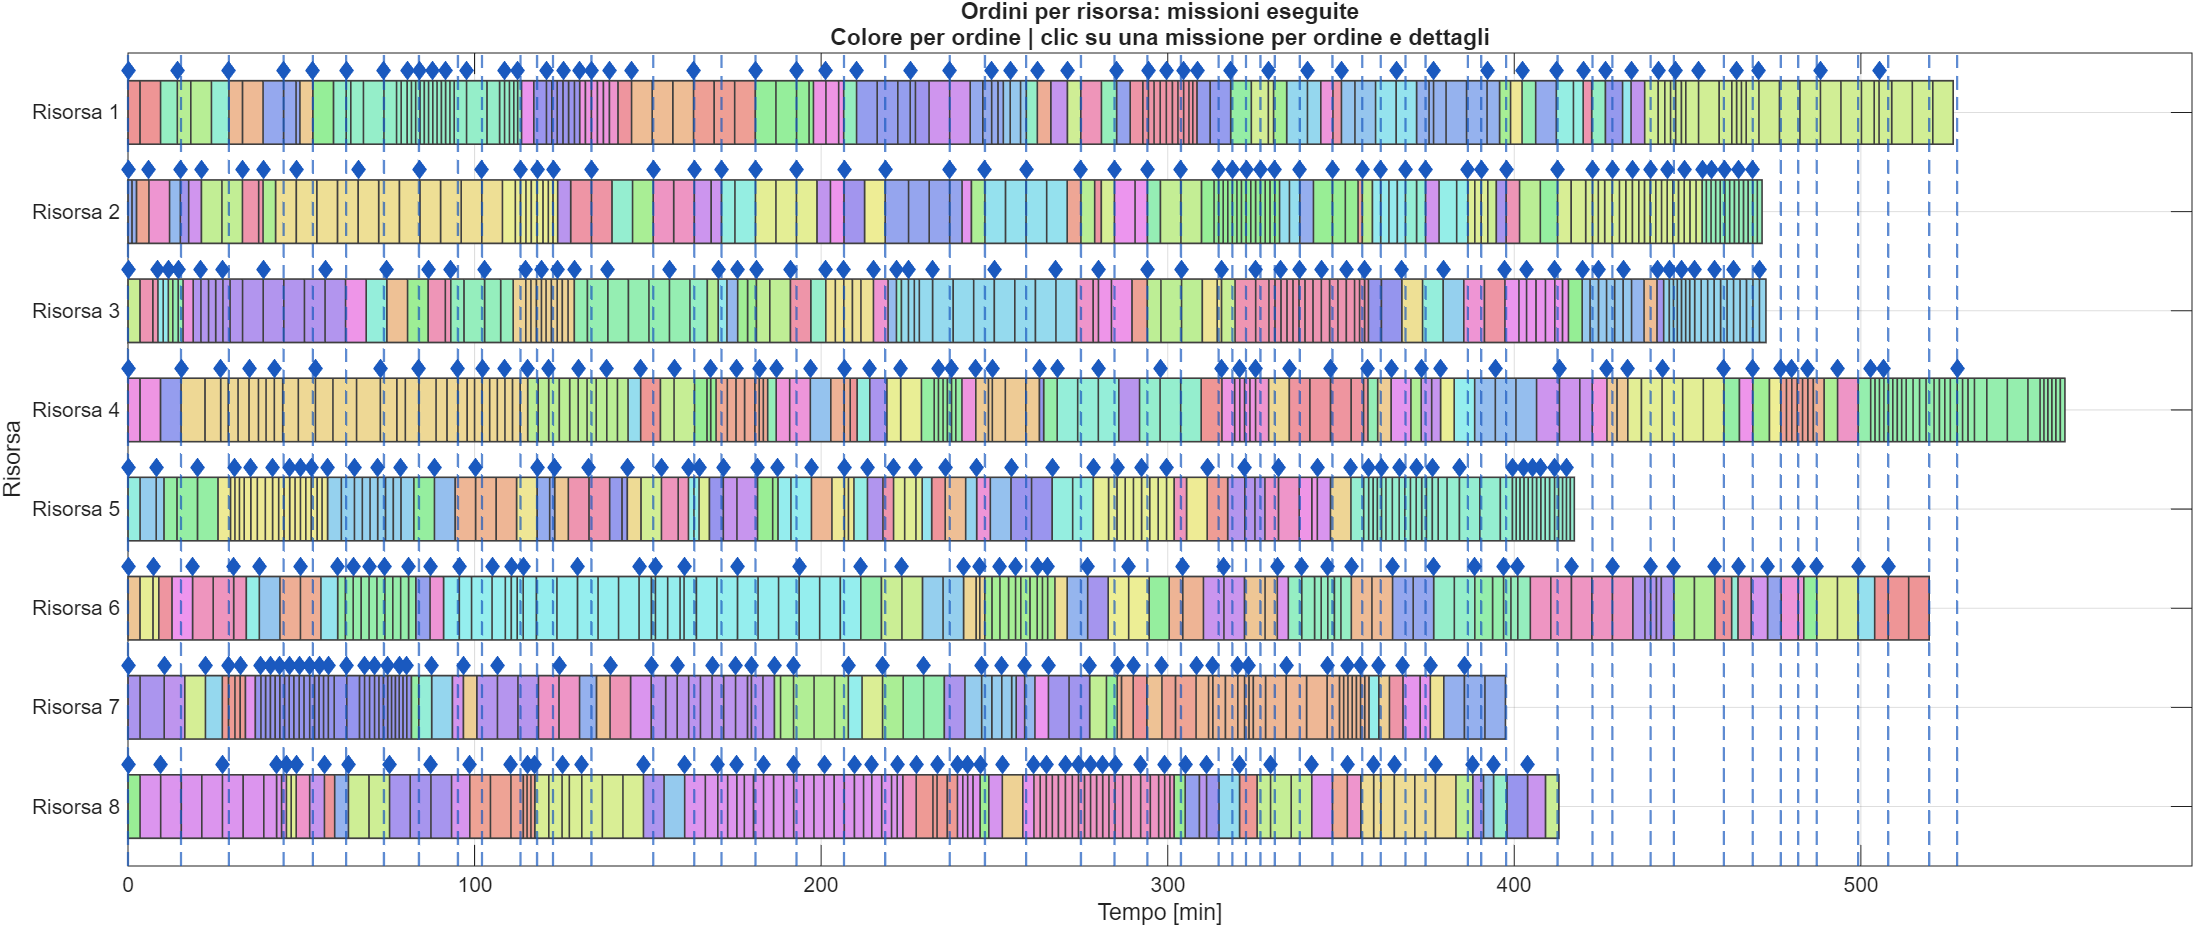
\includegraphics[width=\linewidth]{imgs/esempi/20missioniFIX}
	\caption{Simulazione con assegnazione naive e lotti da 20 missioni.}
	\label{fig:20missionifix}
\end{figure}

\subsection{Prova con 40 missioni}
Con 40 missioni per lotto, il numero di richiami dello scheduler si riduce rispetto alla configurazione precedente. A parità di missioni complessive, il raddoppio della dimensione nominale del lotto comporta indicativamente un dimezzamento del numero di lotti da gestire; il rapporto effettivo dipende dalla composizione degli ordini e dall'eventuale lotto finale incompleto.

Il tempo di esecuzione in MATLAB scende a 156.008 secondi, con una riduzione di circa 6.95 secondi rispetto alla prova con 20 missioni. Questa singola osservazione non consente tuttavia di attribuire la riduzione esclusivamente al minor numero di richiami dello scheduler.

Le ore di lavoro delle risorse diverse dalla 2 sono comprese tra 6.9086 e 8.0386 ore. La risorsa 2 raggiunge invece 9.8656 ore, determinando un makespan simulato di 9.87 ore, superiore a quello della configurazione precedente. Pertanto, la maggiore uniformità osservata per una parte delle risorse non si traduce in una riduzione del tempo complessivo di completamento. La Figura~\ref{fig:40missionifix} riporta la simulazione corrispondente.

\begin{figure}[htbp]
	\centering
	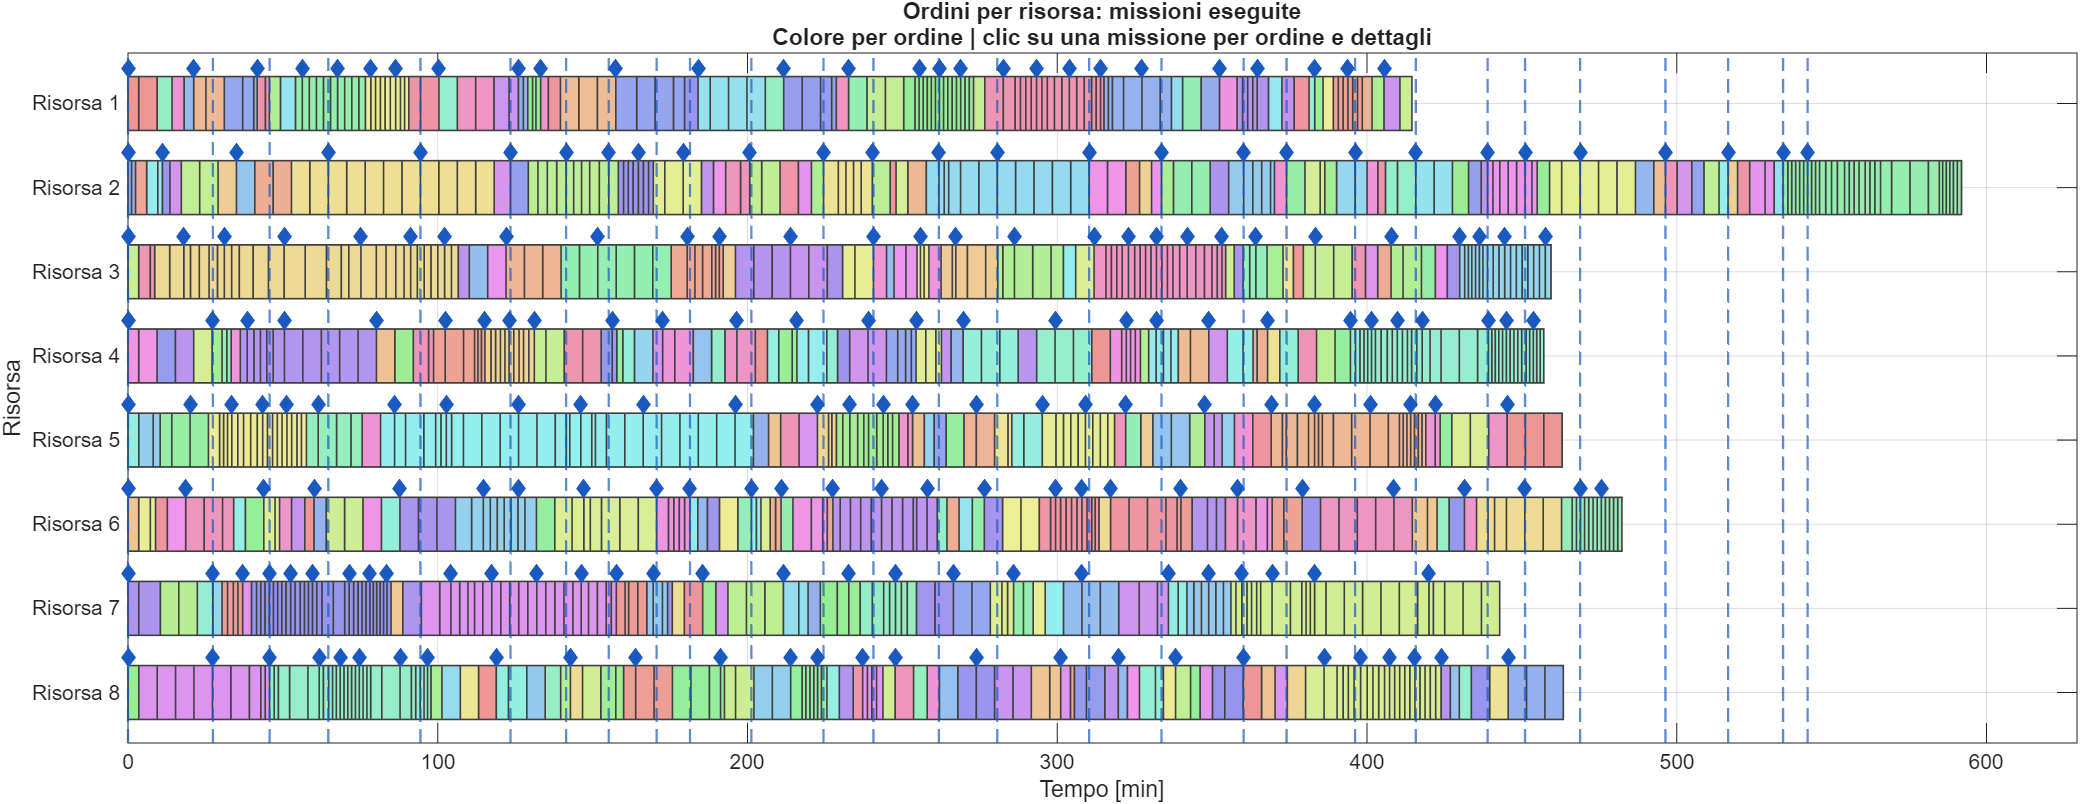
\includegraphics[width=\linewidth]{imgs/esempi/40missioniFIX}
	\caption{Simulazione con assegnazione naive e lotti da 40 missioni.}
	\label{fig:40missionifix}
\end{figure}

\subsection{Prova con 60 missioni}
Con 60 missioni per lotto, il numero nominale di lotti da gestire è circa un terzo rispetto al caso con 20 missioni, a parità di missioni complessive. Anche in questo caso, il numero effettivo di richiami dipende dalla composizione dei lotti.

Il tempo di esecuzione in MATLAB è pari a 156.742 secondi e rimane vicino a quello della prova con 40 missioni. Le ore di lavoro variano da 6.3925 per la risorsa 7 a 9.2633 per la risorsa 4. Il makespan simulato è pari a 9.26 ore, il valore più basso tra le tre prove, sebbene la differenza rispetto al caso con 20 missioni sia contenuta.

L'aumento del numero di missioni per lotto non determina quindi un peggioramento sistematico del makespan. Permane, tuttavia, una distribuzione non uniforme del carico, coerente con l'assenza di un criterio esplicito di bilanciamento nell'assegnazione naive. La Figura~\ref{fig:60missionifix} mostra il risultato della prova.

\begin{figure}[htbp]
	\centering
	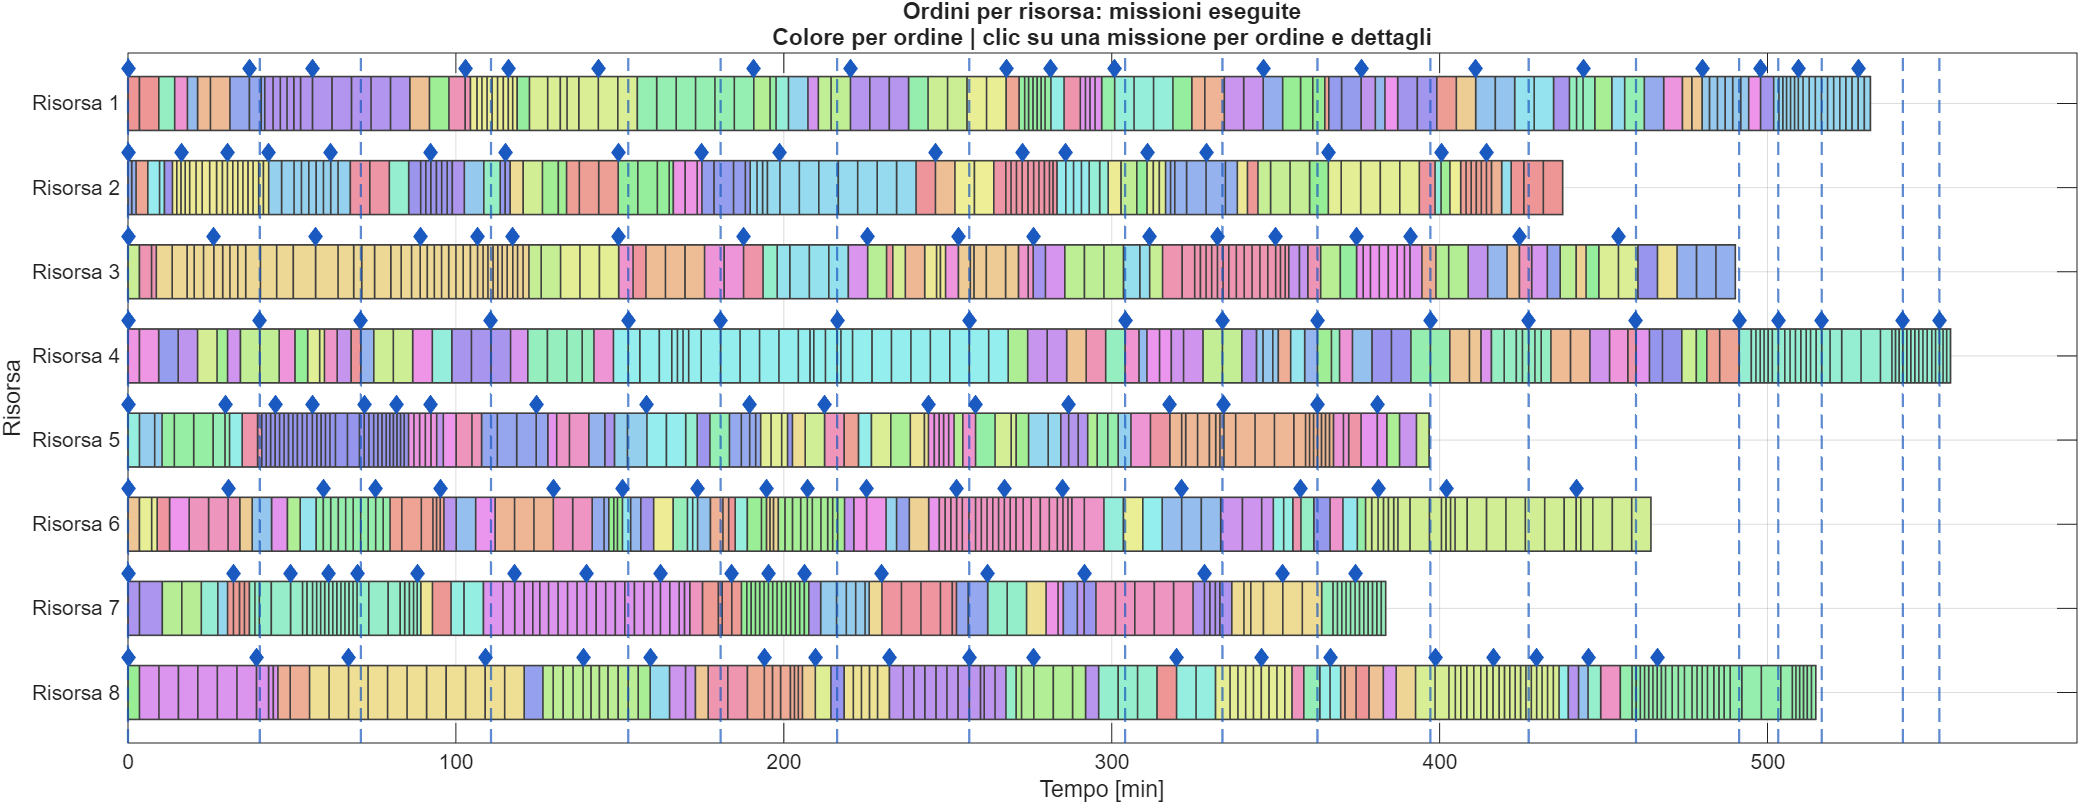
\includegraphics[width=\linewidth]{imgs/esempi/60missioniFIX}
	\caption{Simulazione con assegnazione naive e lotti da 60 missioni.}
	\label{fig:60missionifix}
\end{figure}

\subsection{Confronto dei risultati}
La Tabella~\ref{tab:naive-ore-risorse} riporta le ore di lavoro di ciascuna risorsa nelle tre configurazioni, mentre la Tabella~\ref{tab:naive-riepilogo} sintetizza i tempi di esecuzione e i makespan simulati.

\begin{table}[htbp]
	\centering
	\begin{tabular}{crrr}
		\toprule
		Risorsa & 20 missioni & 40 missioni & 60 missioni \\
		\midrule
		1 & 8.7775 & 6.9086 & 8.8561 \\
		2 & 7.8581 & 9.8656 & 7.2922 \\
		3 & 7.8767 & 7.6569 & 8.1697 \\
		4 & 9.3147 & 7.6181 & 9.2633 \\
		5 & 6.9553 & 7.7167 & 6.6133 \\
		6 & 8.6619 & 8.0386 & 7.7408 \\
		7 & 6.6242 & 7.3806 & 6.3925 \\
		8 & 6.8811 & 7.7231 & 8.5789 \\
		\bottomrule
	\end{tabular}
	
	\caption{Ore di lavoro delle risorse nelle prove con assegnazione naive.}
	\label{tab:naive-ore-risorse}
\end{table}

\begin{table}[htbp]
	\centering
	\caption{Confronto tra tempo di esecuzione in MATLAB e makespan simulato.}
	\label{tab:naive-riepilogo}
	\begin{tabular}{crr}
		\toprule
		Missioni per lotto & Tempo MATLAB (s) & Makespan (h) \\
		\midrule
		20 & 162.962 & 9.31 \\
		40 & 156.008 & 9.87 \\
		60 & 156.742 & 9.26 \\
		\bottomrule
	\end{tabular}
\end{table}

Le differenze tra il massimo e il minimo delle ore di lavoro sono pari a circa 2.69, 2.96 e 2.87 ore, rispettivamente per i lotti da 20, 40 e 60 missioni. Secondo questo indicatore, nessuna delle due configurazioni con lotti più grandi migliora il bilanciamento rispetto alla prova con 20 missioni.

I risultati mostrano che la dimensione del lotto influenza sia la distribuzione del carico sia il makespan, senza evidenziare un andamento monotono. Nelle prove riportate, il lotto da 40 missioni presenta il minor tempo di esecuzione in MATLAB, mentre quello da 60 missioni produce il minor makespan simulato. Queste osservazioni descrivono le esecuzioni considerate e non sono sufficienti, da sole, a stabilire quale dimensione del lotto sia preferibile in generale.



\chapter{Conclusions}




\printbibliography

\end{document}
